\documentclass[12pt,a4paper]{report}
\usepackage[utf8]{vietnam}
\usepackage{amsmath, amsthm, amssymb,latexsym,amscd,amsfonts,enumerate}
\usepackage[top=3.5cm, bottom=3.0cm, left=3.5cm, right=2.0cm]{geometry}
\usepackage{color, fancyhdr, graphicx, wrapfig}
\usepackage[unicode]{hyperref}
\usepackage{indentfirst}
\usepackage{tcolorbox}
\usepackage{caption}
\usepackage{subcaption}

\newtheorem{dn}{Định nghĩa}[section]
\newtheorem{tc}[dn]{Tính chất}
\newtheorem{dl}[dn]{Định lí}
\newtheorem{md}[dn]{Mệnh đề}
\newtheorem{bd}[dn]{Bổ đề}
\newtheorem{hq}[dn]{Hệ quả}
\newtheorem{nx}[dn]{Nhận xét}
\newtheorem{vd}{Ví dụ}

\pagenumbering{roman}\pagestyle{plain}
\pagestyle{fancy}
\lhead{\it Viện Toán Ứng Dụng và Tin Học}
\rhead{\it Đại học Bách Khoa Hà Nội}
\lfoot{\it Báo cáo cuối kỳ}
\rfoot{\it Toán - Tin 02 khóa 64}
\renewcommand{\headrulewidth}{1,2pt} 			
\renewcommand{\footrulewidth}{1,2pt}   % Cái này là tiêu đề chạy



\begin{document} 

\fontsize{13pt}{18pt}\selectfont   % Lệnh thay đổi cỡ chữ thành cỡ 13, cỡ dòng 18 (theo quy chuẩn của Khóa Luận TN).

\setlength{\baselineskip}{18truept}
\begin{titlepage}                                                       % Đây là trang bìa
\begin{center}
{\large\bf TRƯỜNG ĐẠI HỌC BÁCH KHOA HÀ NỘI}\\
{\large\bf VIỆN TOÁN ỨNG DỤNG VÀ TIN HỌC} \\
{---------------------o0o--------------------}
\vskip 1cm

\includegraphics[scale=0.4]{Figures/HUST}
\vskip 2cm
{\bf BÁO CÁO CUỐI KỲ}\\[1cm]
{\Large\bf \textbf{Một số bài tập trên Alchemi .NET Framework}}\\
\vskip 1cm
{\bf {\it Học phần:}  Tính toán song song}
\vskip 2cm

\begin{tabular}{r l}
Giảng viên hướng dẫn:&{\bf TS. ĐOÀN DUY TRUNG}\\[0.5cm]
Sinh viên:&{\bf Nguyễn Công Hiếu - 20195016}\\[0.5cm]
Lớp:&{\bf Toán tin 02 - khóa 64}
\end{tabular}
\vfill
{\bf HÀ NỘI, 01/2022}
\end{center}
\end{titlepage}



\chapter*{Lời nói đầu}
\addcontentsline{toc}{chapter}{{\bf  Lời nói đầu}\rm} %Đưa lời nói đầu vào mục lục
Xã hội đang ngày càng phát triển nhanh chóng hơn bao giờ hết, đòi hỏi con người phải giải quyết những bài toán lớn và phức tạp trên nhiều lĩnh vực từ khoa học kỹ thuật như lượng tử, khí hậu, môi trường, vũ trụ hàng không, sinh học tế bào, cho đến kinh tế xã hội như ngân hàng, điện toán, ... Chúng là những bài toán mà từ lâu đã luôn là thách thức đối với nhân loại, song chỉ trong khoảng 1, 2 thập kỷ trở lại đây, chúng ta mới có được những kỹ thuật hay thuật toán để từng bước hoàn thiện các lời giải. Tuy nhiên, khối lượng dữ liệu cho các bài toán ngày một phình to khiến cho chỉ một chiếc máy tính là không đủ. Từ đó, các nhà khoa học đã đưa ra một giải pháp, đó là tính toán song song trên lưới với mỗi chiếc một chiếc máy tính có thể kết nối với nhau thông qua mạng và xử lý các bài toán con trên các nút của lưới. Một nhóm các nhà nghiên cứu tại Đại học Melbourne đã cùng nhau phát triển Alchemi framework (dựa trên .NET framewwork và chạy trên HĐH Windows) cho phép các lập trình viên có thể dễ dàng tạo ra một lưới tính toán.	\\

Với sự chỉ bảo của thầy Đoàn Duy Trung, em xin phép được trình bày một số bài toán đơn giản được thiết kế để chạy trên lưới Alchemi. Các bài toán sau đây được thực nghiệm trên mô hình Cluster với 1 manager và 1 hoặc nhiều executor. Tuy nhiên do điều kiện không cho phép nên em chỉ có thể cài đặt 1 manager và 1 executor trên cùng 1 máy.

\tableofcontents	                        % Lệnh mục lục


\chapter{Số chính phương}
\pagenumbering{arabic}                      % Đánh lại trang

\begin{tcolorbox}[title=Đề bài, colback=red!5!white, colframe=red!70!black]
Liệt kê các số chính phương từ 1 đến n, với n nhập từ bàn phím. Phân chia đoạn [1,n] thành các đoạn để chạy trên các Executor trong lưới.
\end{tcolorbox}

\begin{center}
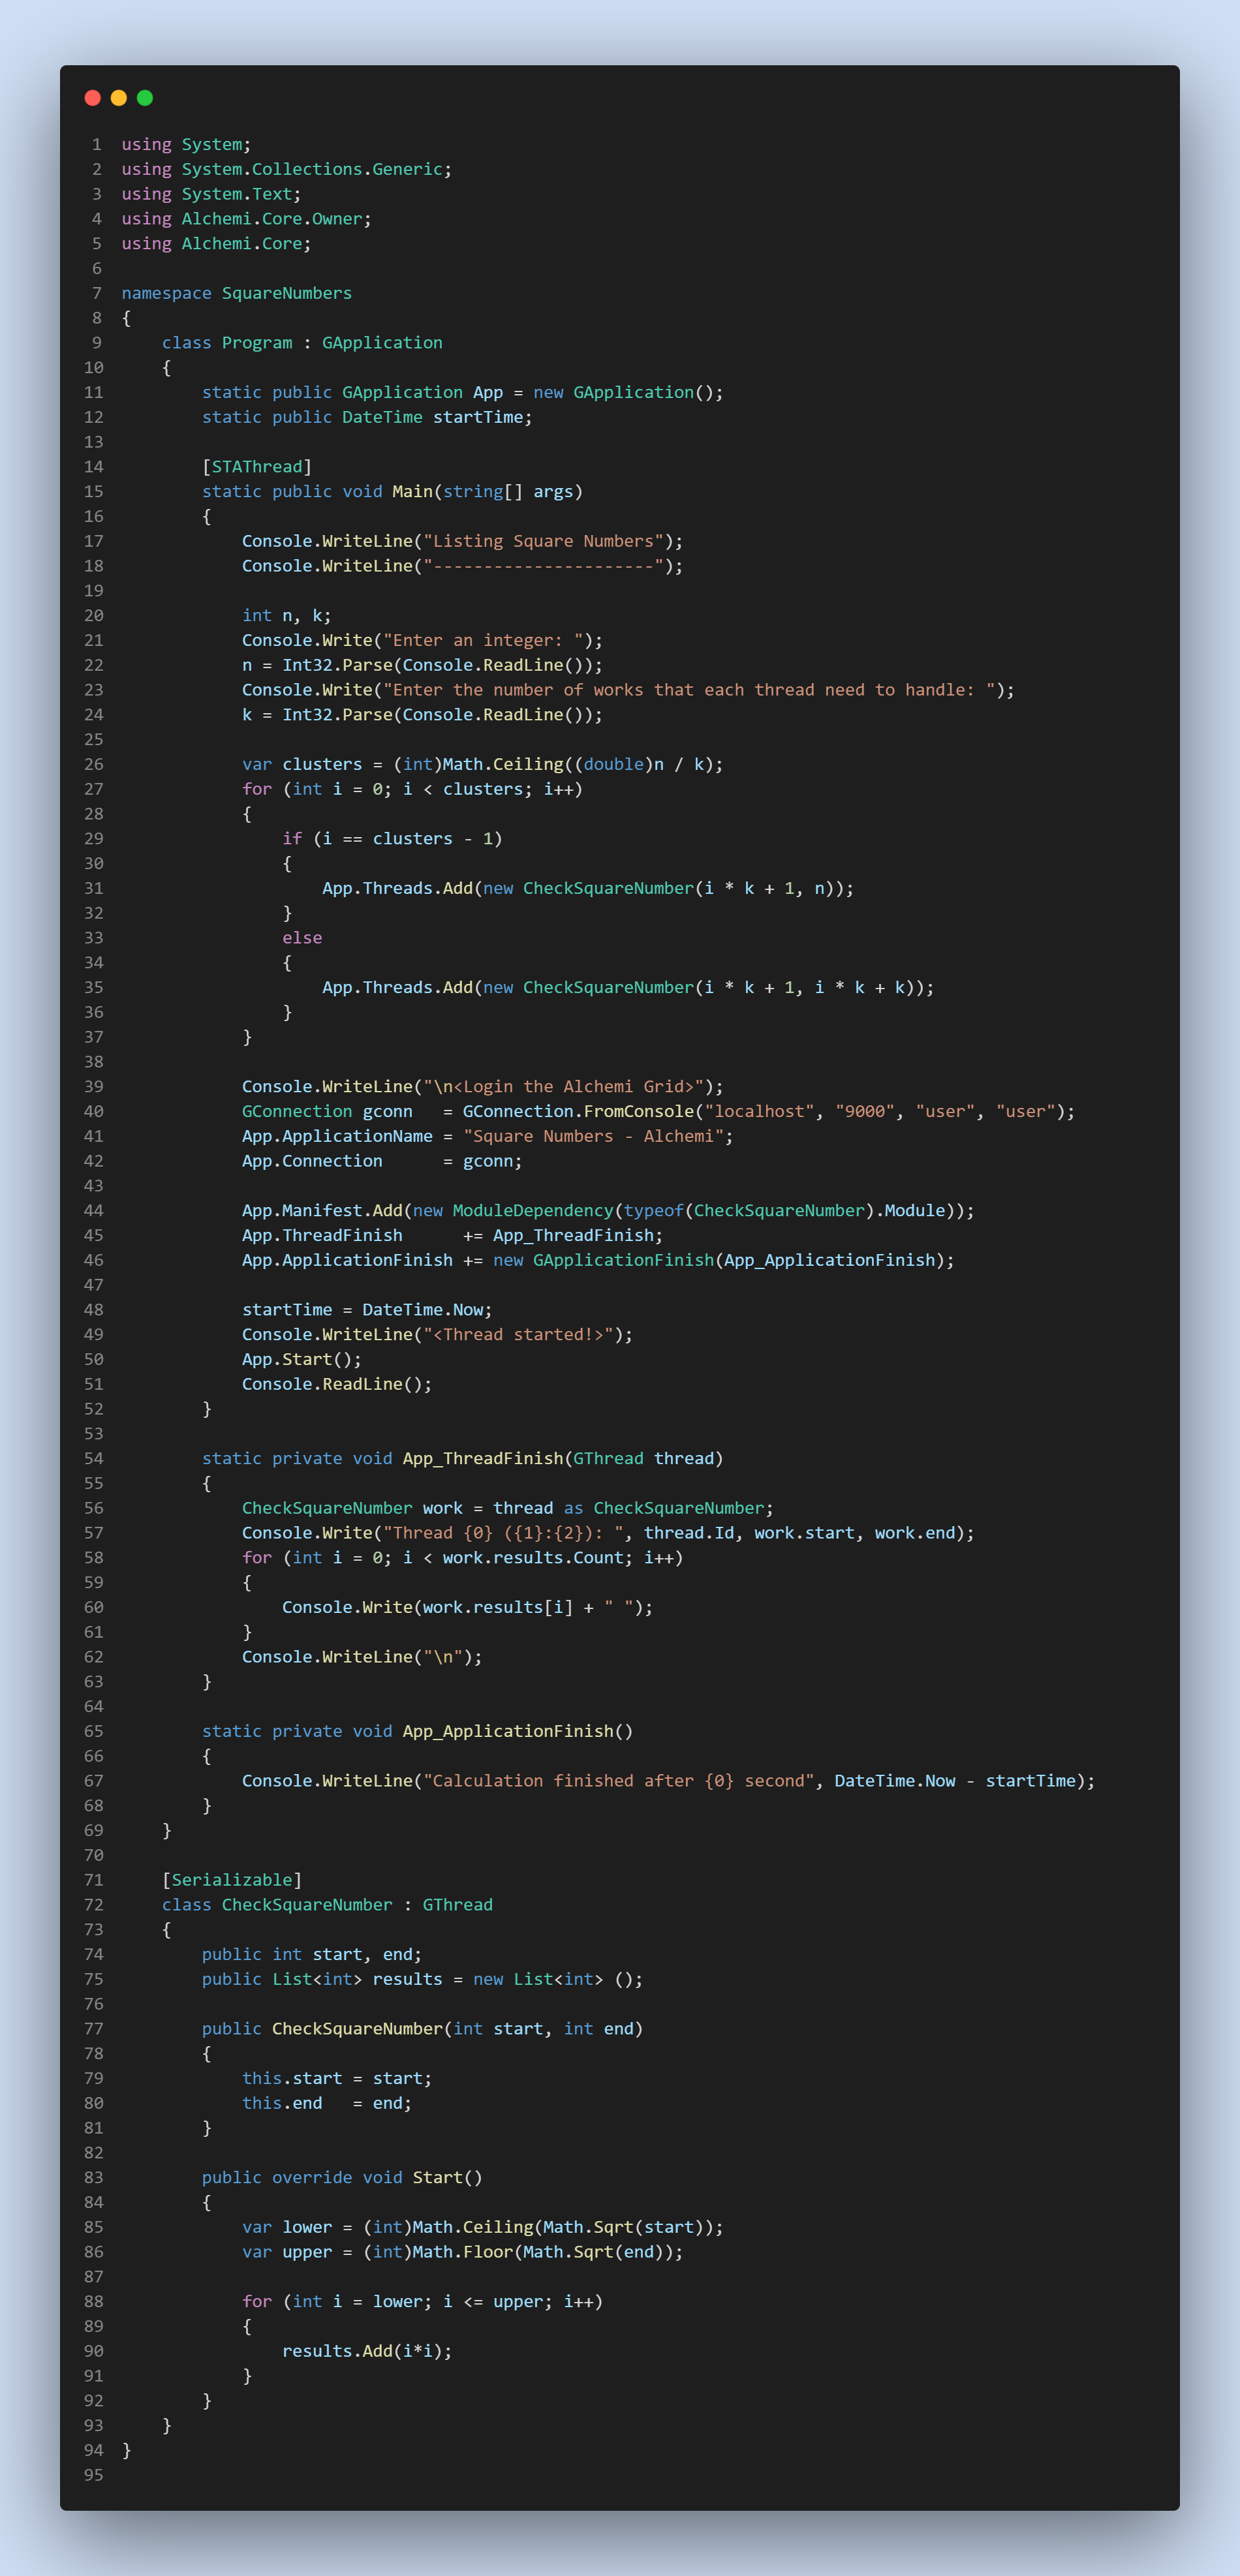
\includegraphics[trim=0in 32in 0in 0in, clip, scale=.23]{./Figures/SquareNumbers/SquareNumbers}
\clearpage
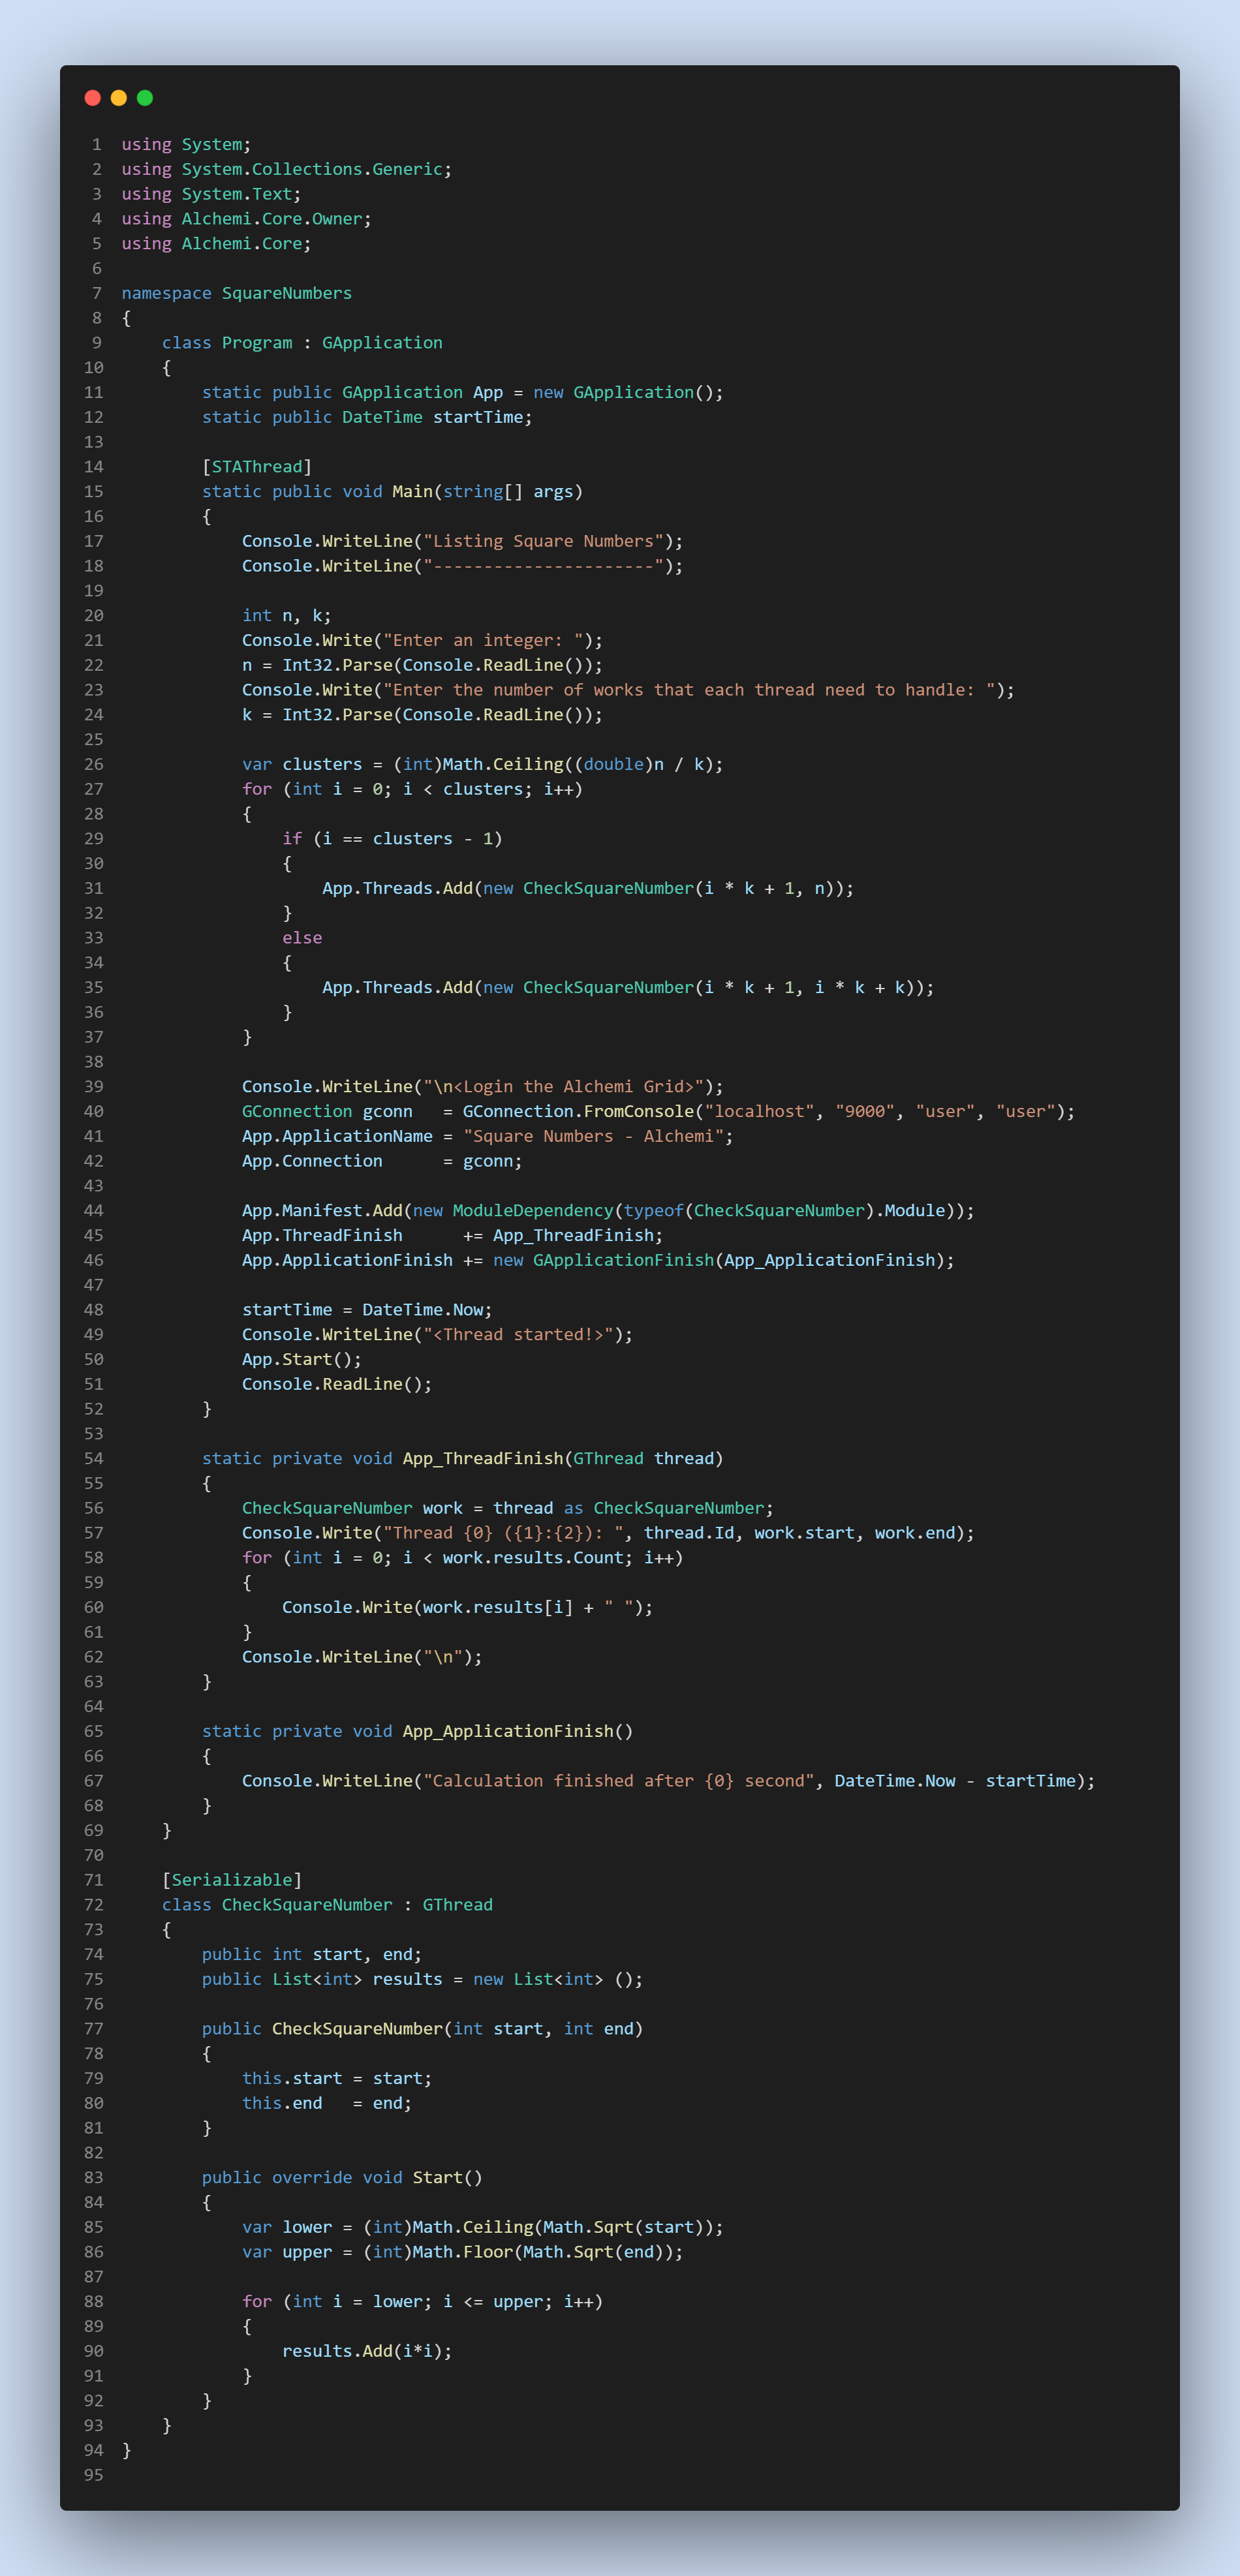
\includegraphics[trim=0in 0in 0in 22.8in, clip, scale=.23]{./Figures/SquareNumbers/SquareNumbers}
\clearpage
\end{center}

\section{Kết quả tính toán}
\begin{center}
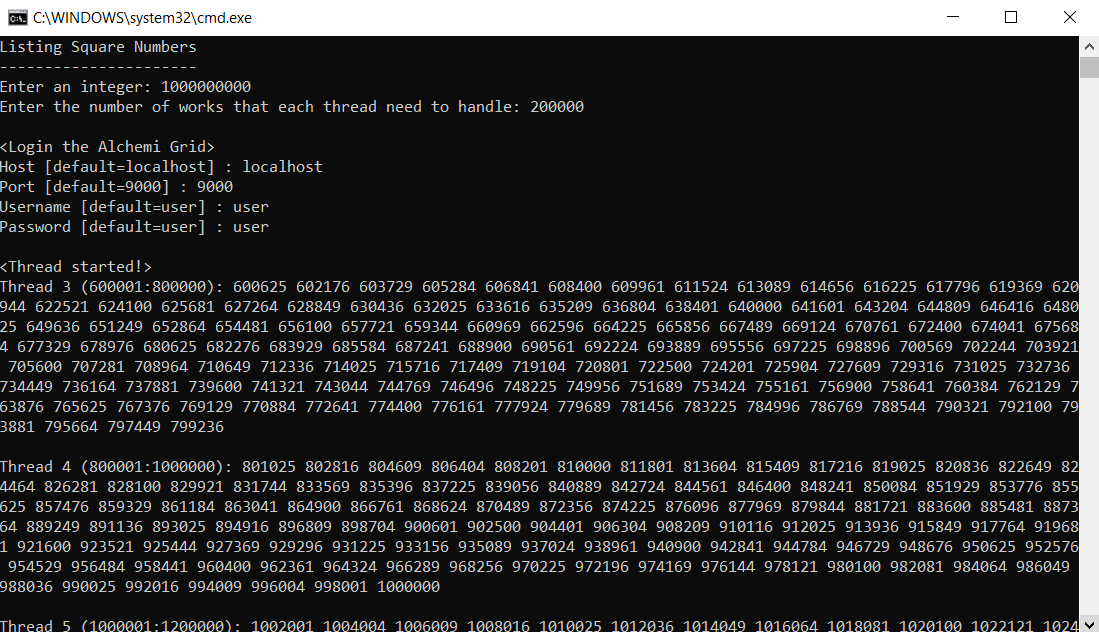
\includegraphics[scale=.6]{./Figures/SquareNumbers/Result_01}
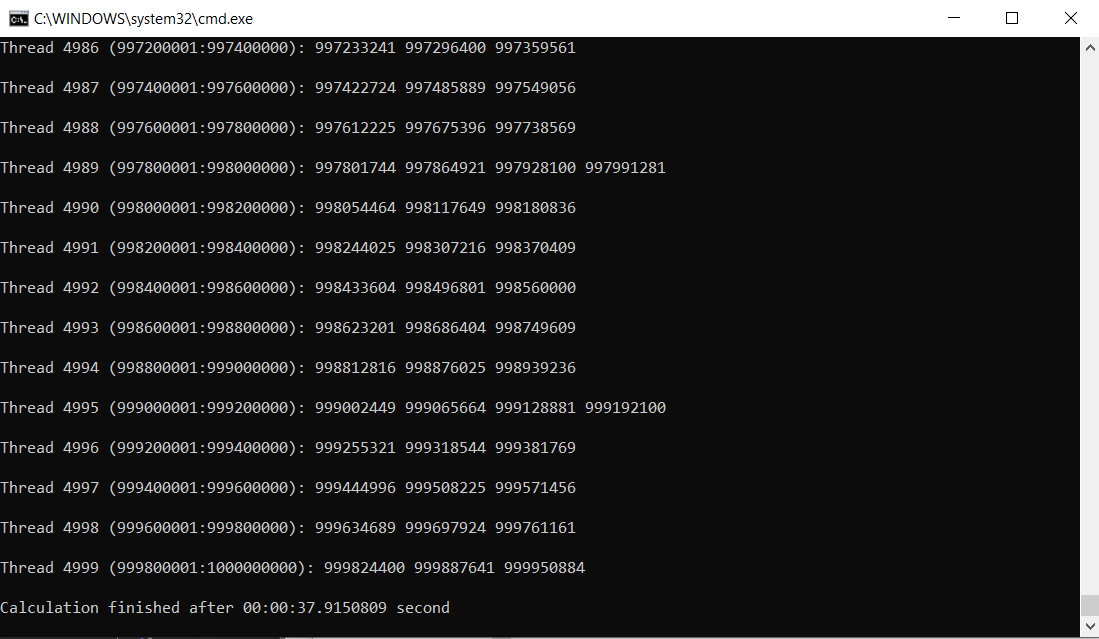
\includegraphics[scale=.6]{./Figures/SquareNumbers/Result_02}
\clearpage
\end{center}

\section{Giao diện Alchemi}
\begin{center}
    \begin{figure}[htp]
    \begin{center}
     	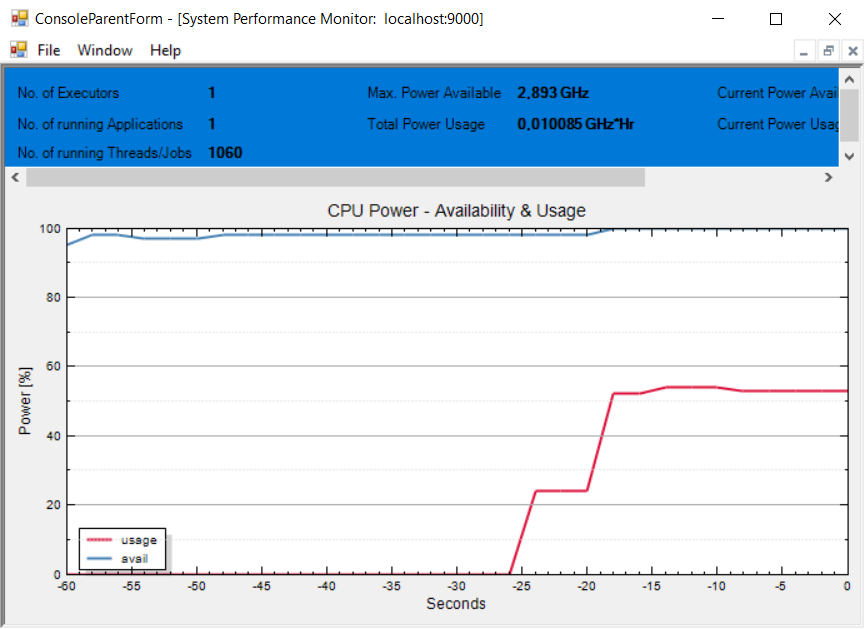
\includegraphics[scale=.6]{./Figures/SquareNumbers/Graph}
     	\caption{Đồ thị đánh giá hiệu năng}
  
     	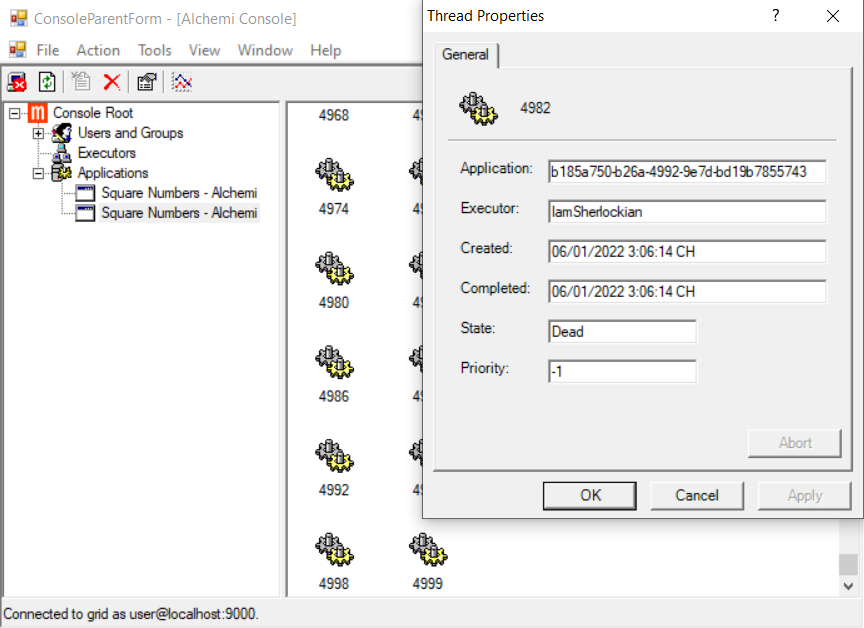
\includegraphics[scale=.6]{./Figures/SquareNumbers/Manage}
    	\caption{Giao diện quản lý luồng trong Alchemi Grid}
    \end{center}
    \end{figure}
\end{center}


\chapter{Tích phân}

\begin{tcolorbox}[title=Đề bài, colback=red!5!white, colframe=red!70!black]
Cho n nhập từ bàn phím. Tính gần đúng tích phân sau:
$$\int_0^n f(x)dx$$
Ở đó, hàm $f(x)$ là tùy ý. Phân chia [0,n] vào các Executor để chạy trong lưới.
\end{tcolorbox}

\begin{center}
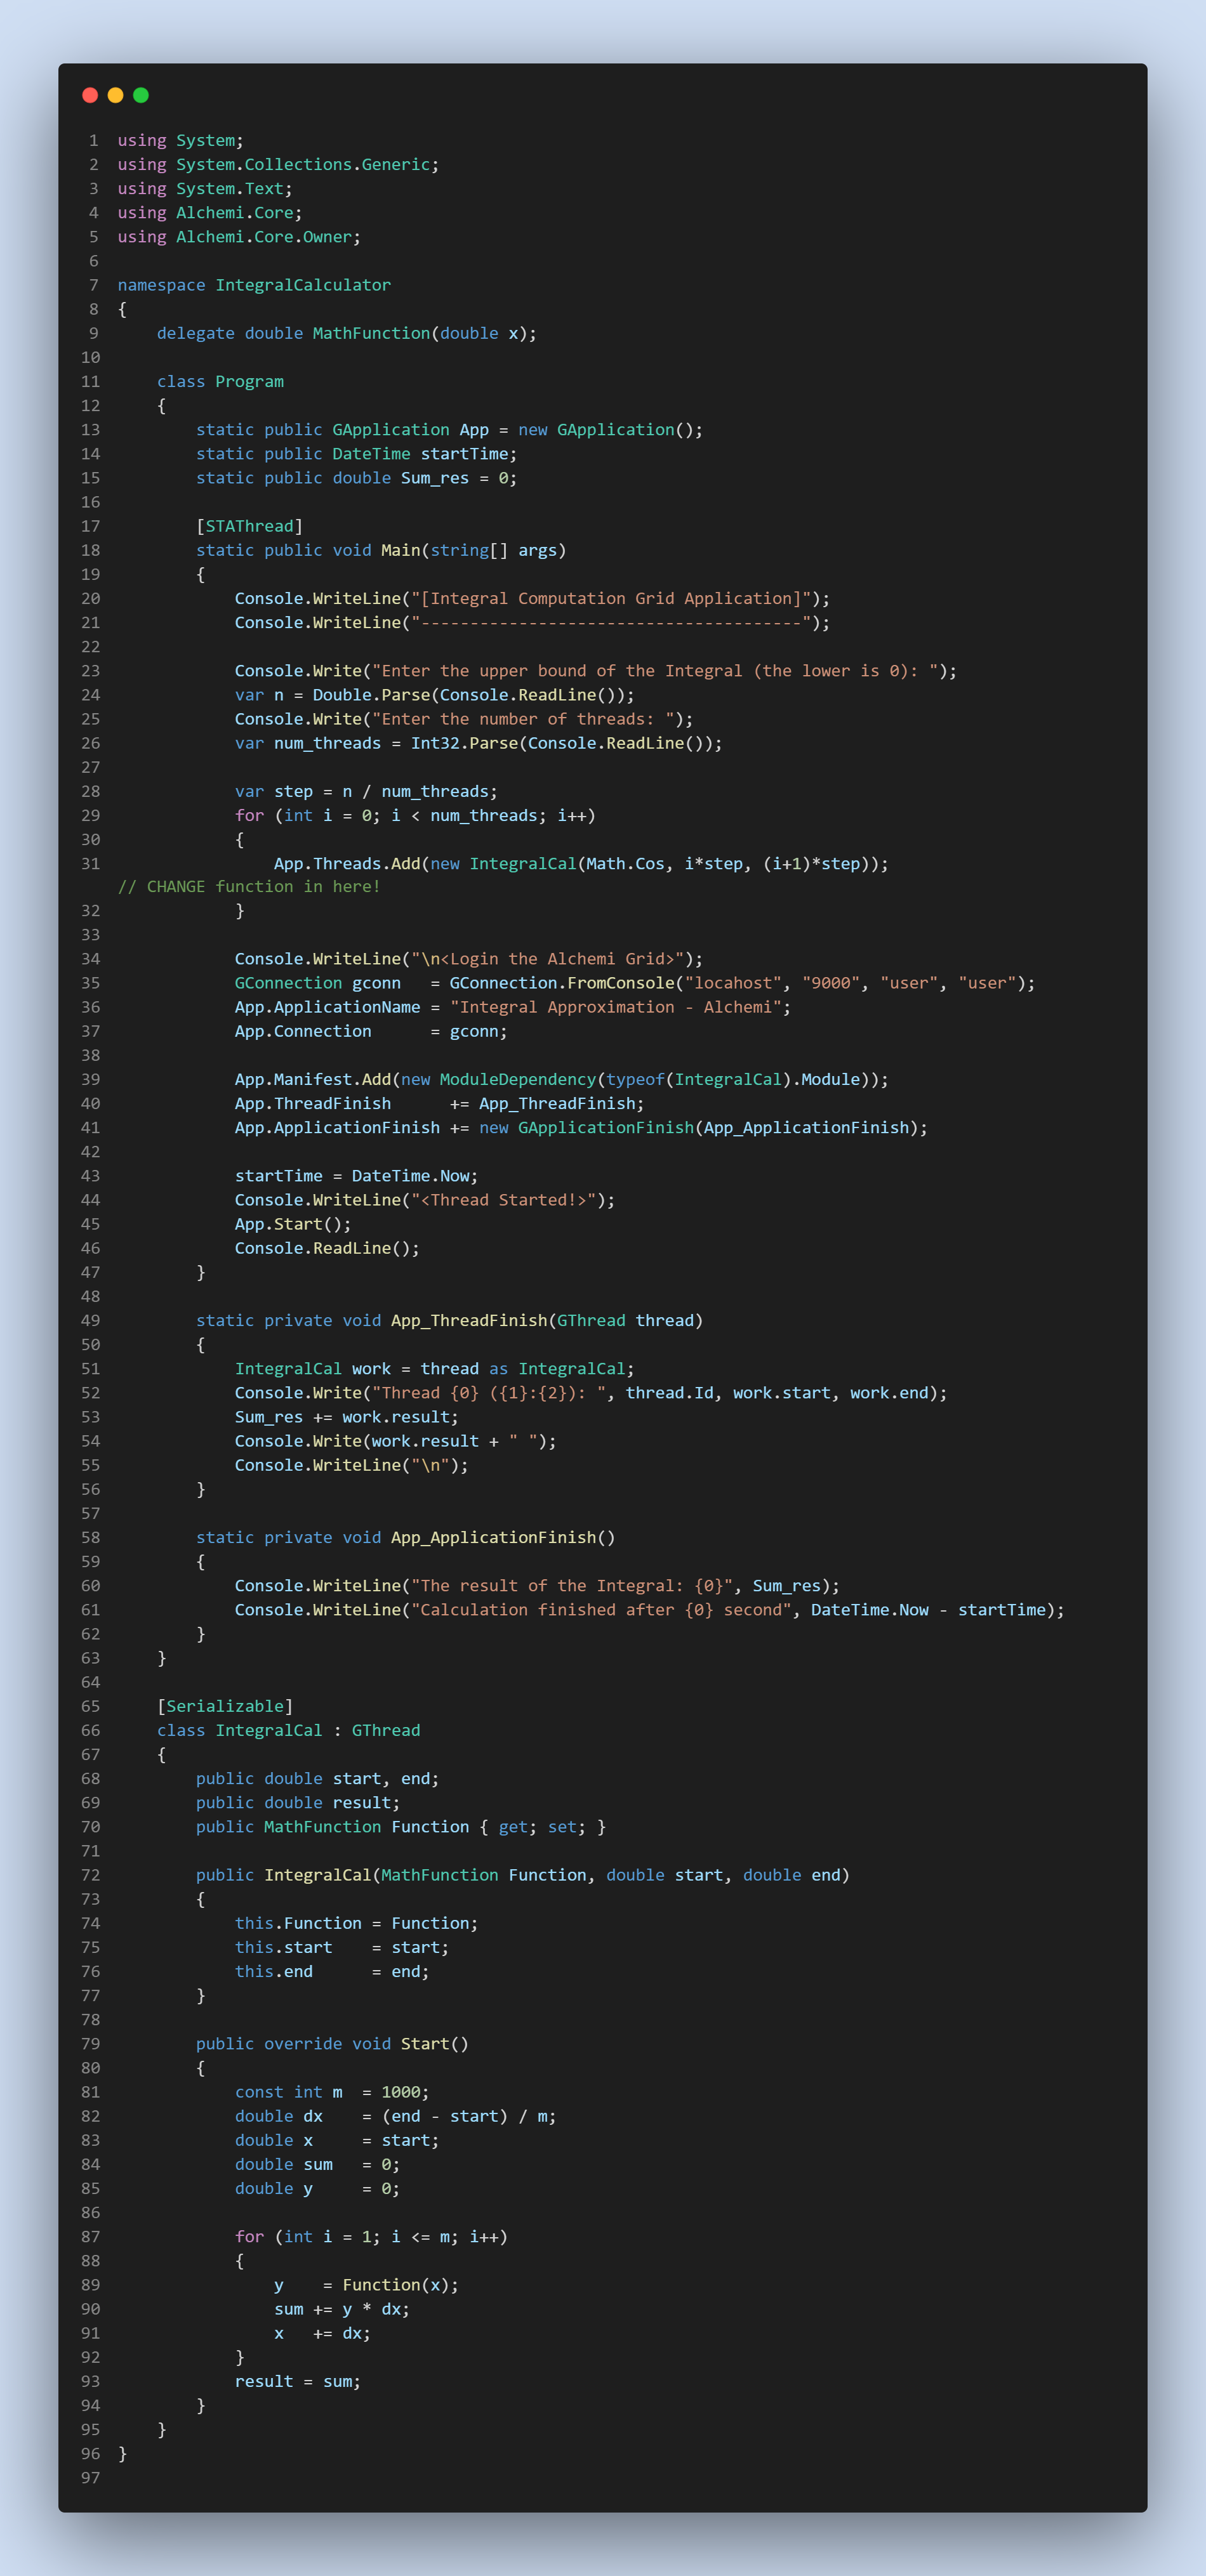
\includegraphics[trim=0in 37.2in 0in 0in, clip, scale=.23]{./Figures/IntegralCalculator/IntegralCalculator}
\clearpage
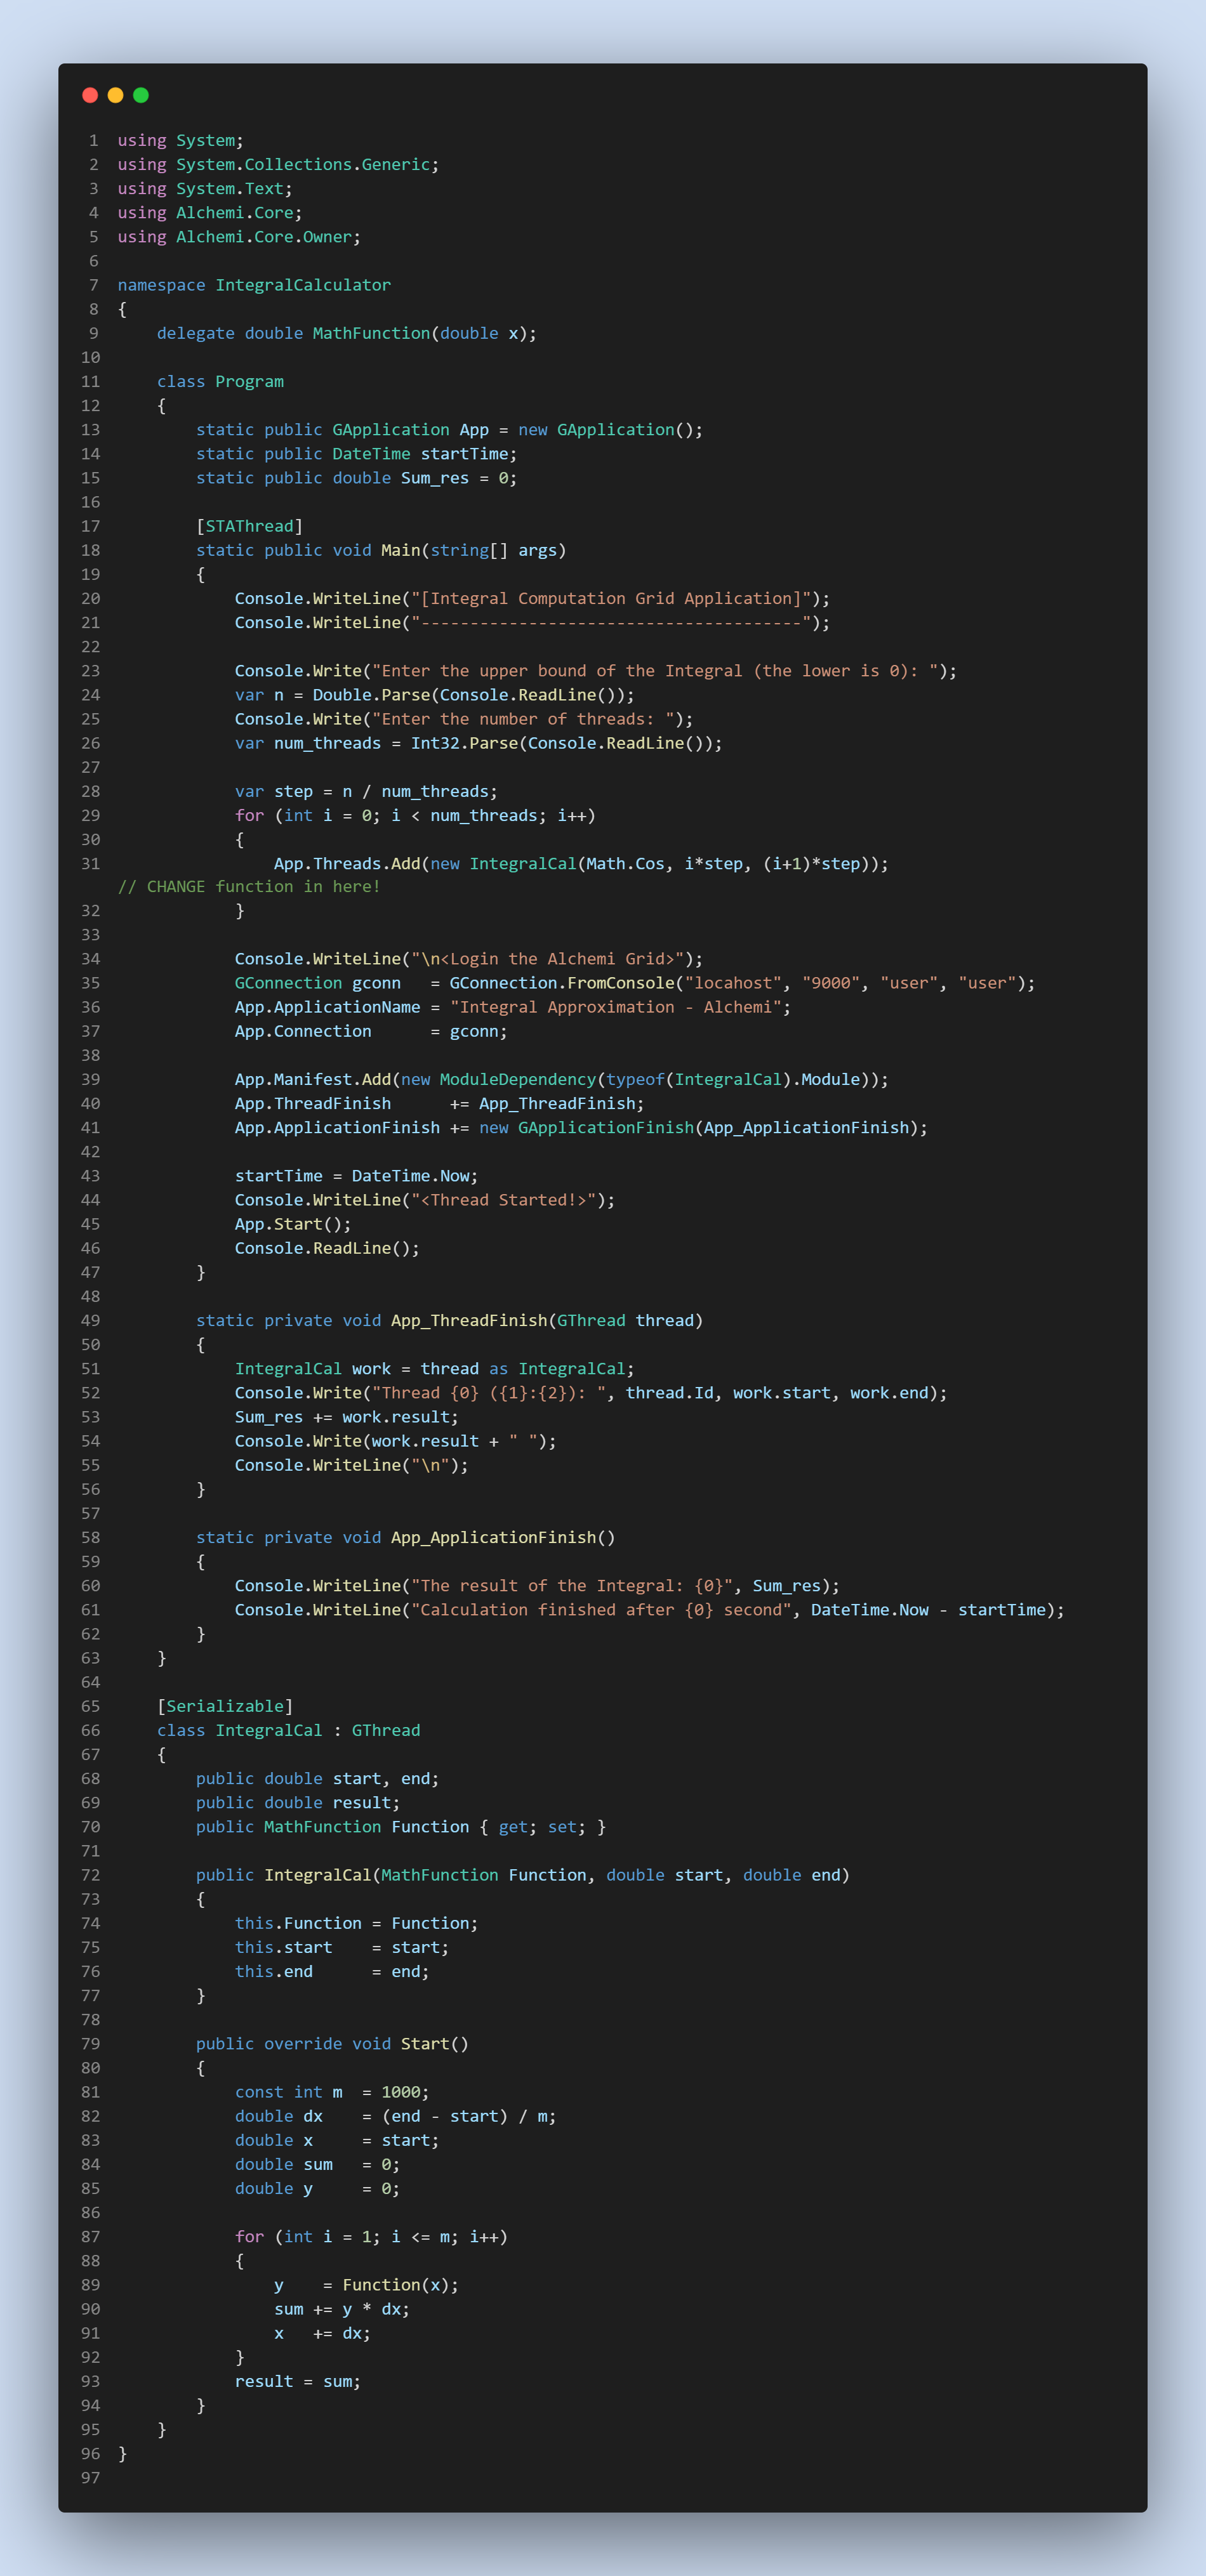
\includegraphics[trim=0in 0in 0in 19.1in, clip, scale=.23]{./Figures/IntegralCalculator/IntegralCalculator}
\clearpage
\end{center}

\section{Kết quả tính toán}
\begin{center}
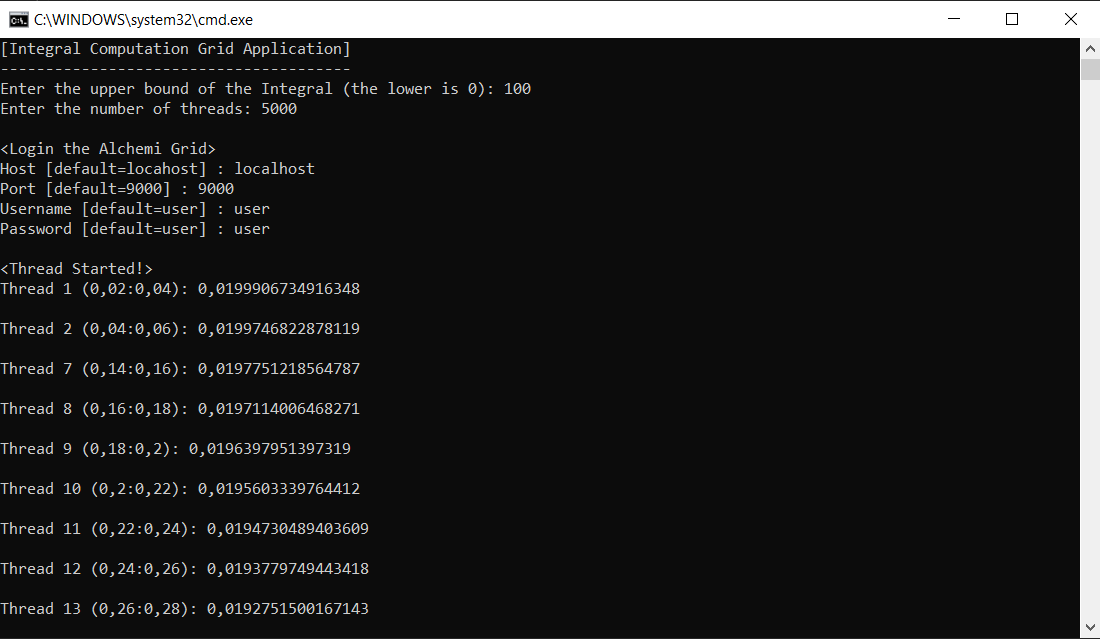
\includegraphics[scale=.6]{./Figures/IntegralCalculator/Result_01}
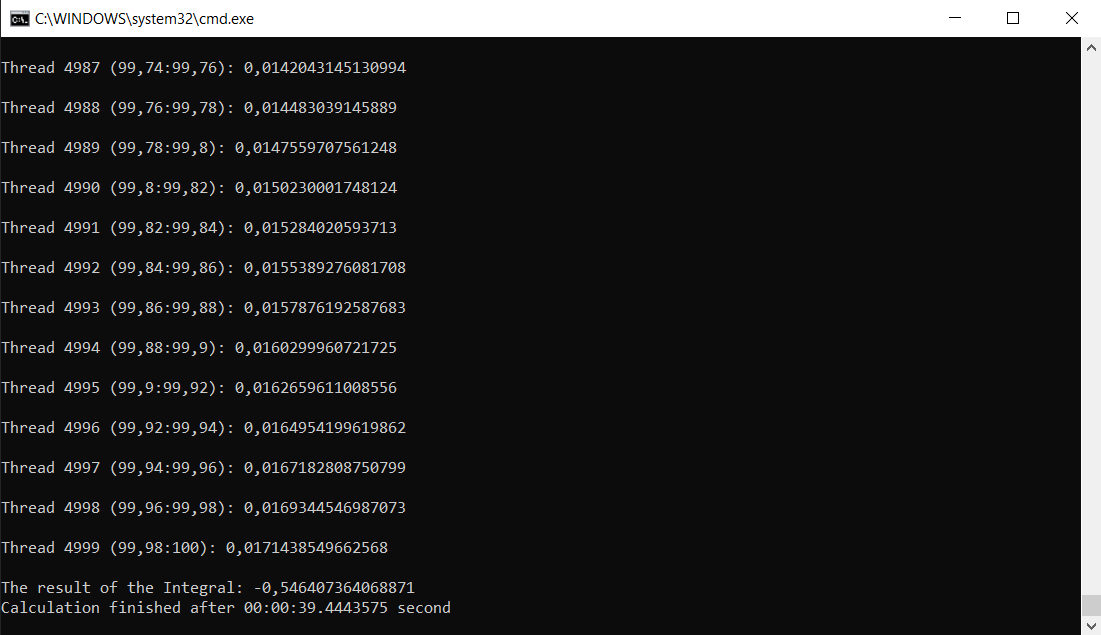
\includegraphics[scale=.6]{./Figures/IntegralCalculator/Result_02}
\end{center}
\clearpage

\section{Giao diện Alchemi}
\begin{center}
    \begin{figure}[htp]
    \begin{center}
     	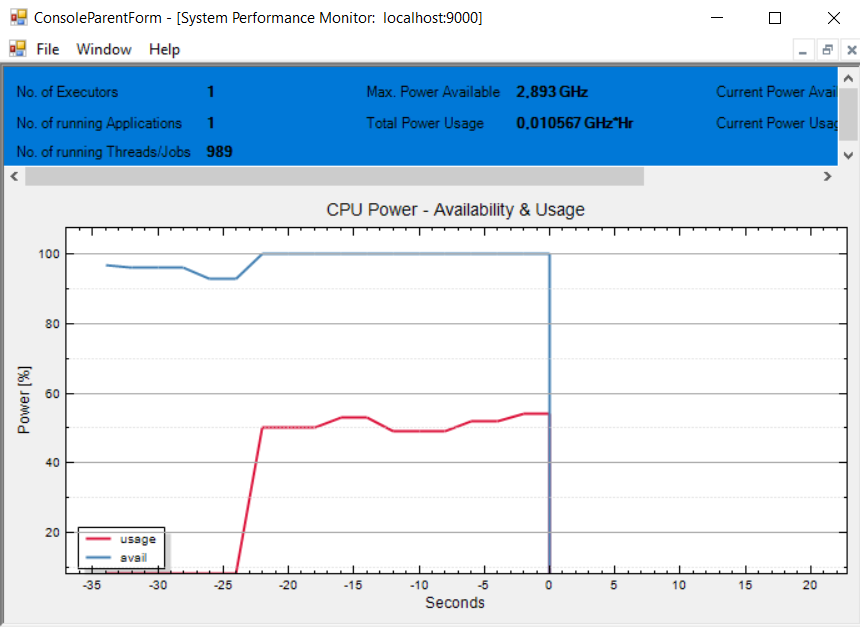
\includegraphics[scale=.6]{./Figures/IntegralCalculator/Graph}
     	\caption{Đồ thị đánh giá hiệu năng}
  
     	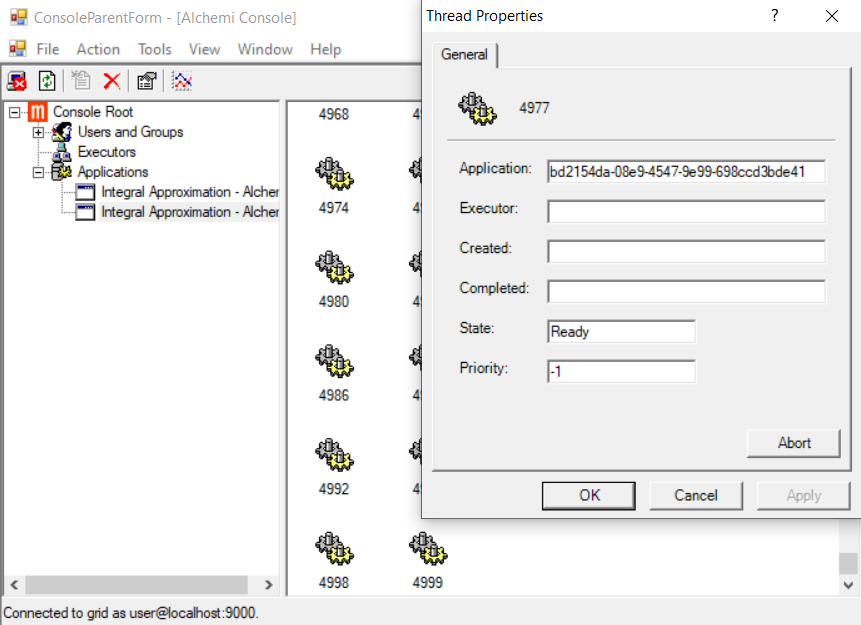
\includegraphics[scale=.6]{./Figures/IntegralCalculator/Manage}
    	\caption{Giao diện quản lý luồng trong Alchemi Grid}
    \end{center}
    \end{figure}
\end{center}

\chapter{Bội chung nhỏ nhất}

\begin{tcolorbox}[title=Đề bài, colback=red!5!white, colframe=red!70!black]
Nhập 1 ma trận cỡ $m$ x $n$, tìm bội số chung nhỏ nhất của từng hàng trong ma trận đó. Yêu cầu, phân chia ma trận thành nhiều ma trận nhỏ hơn với kích thuóc $k$ x $b$, mỗi ma trận nhỏ là 1 luồng và thực hiện trên các nút tính toán.
\end{tcolorbox}

\begin{center}
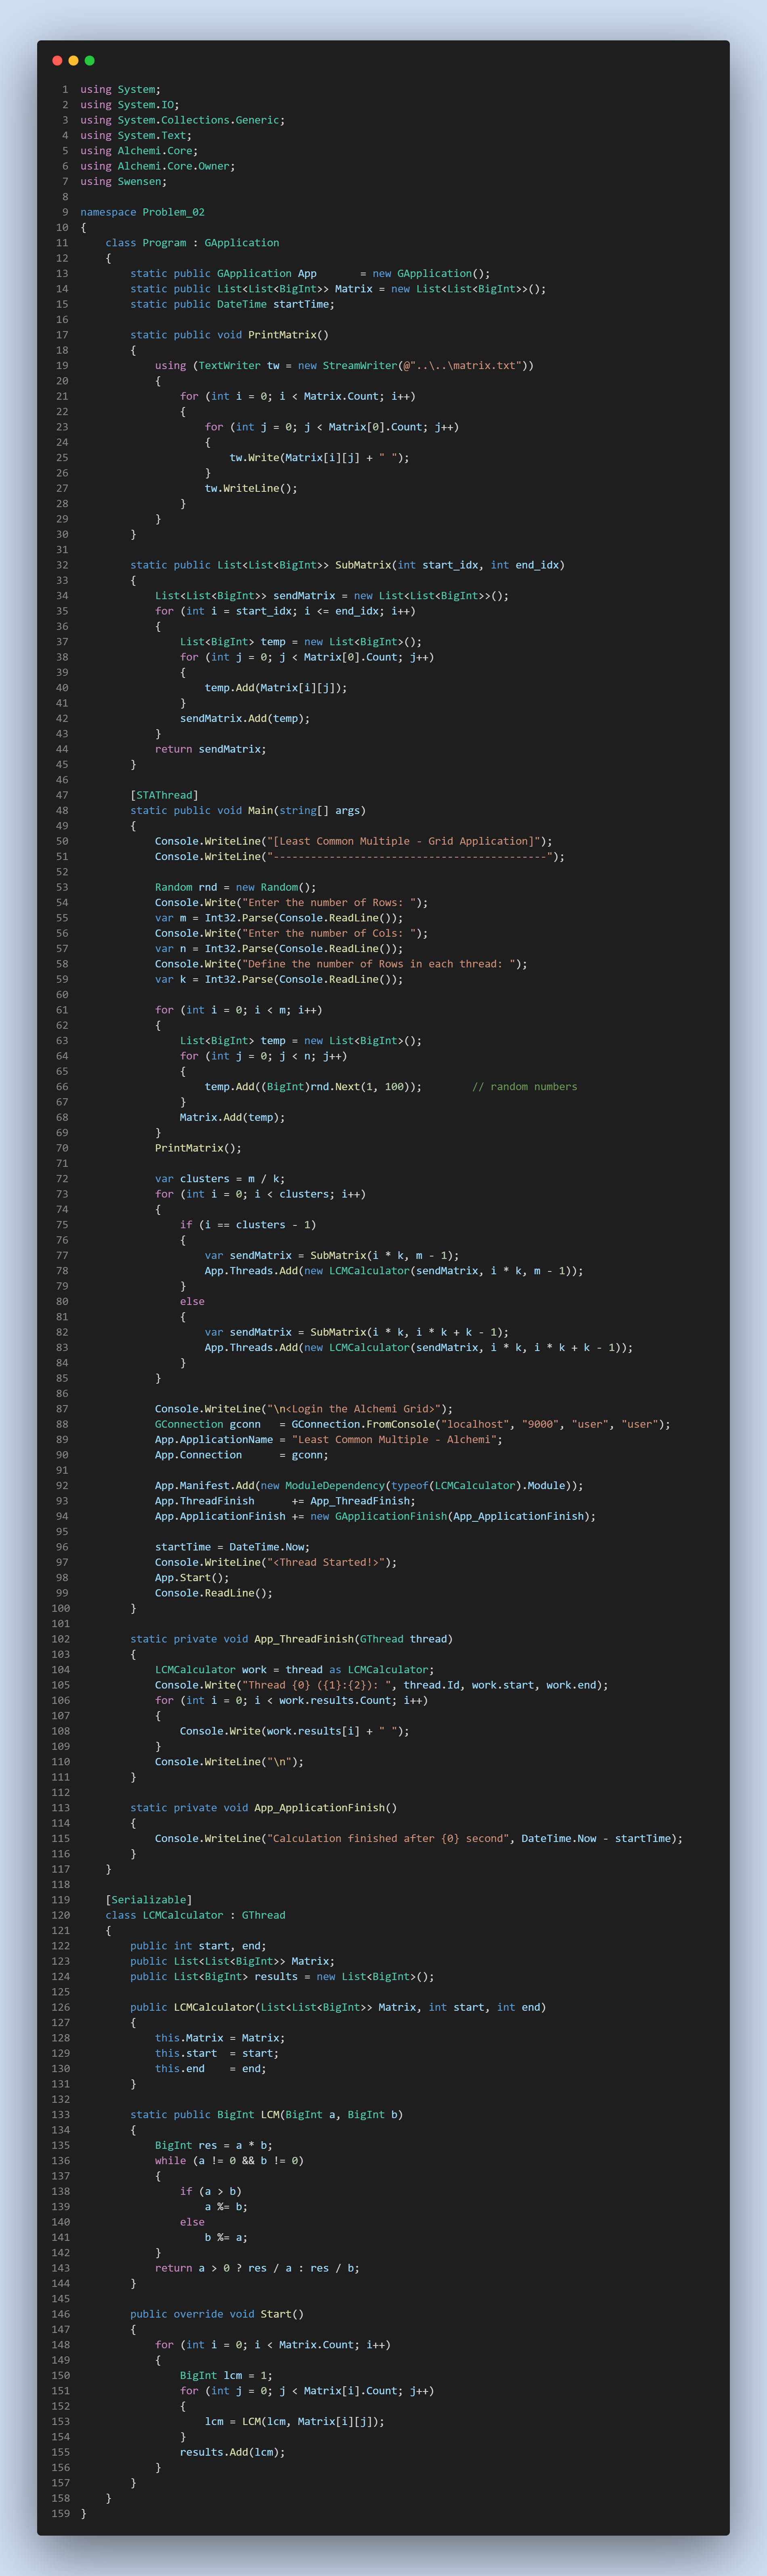
\includegraphics[trim=0in 67.25in 0in 0in, clip, scale=.23]{./Figures/Problem_02/Problem_02}
\clearpage
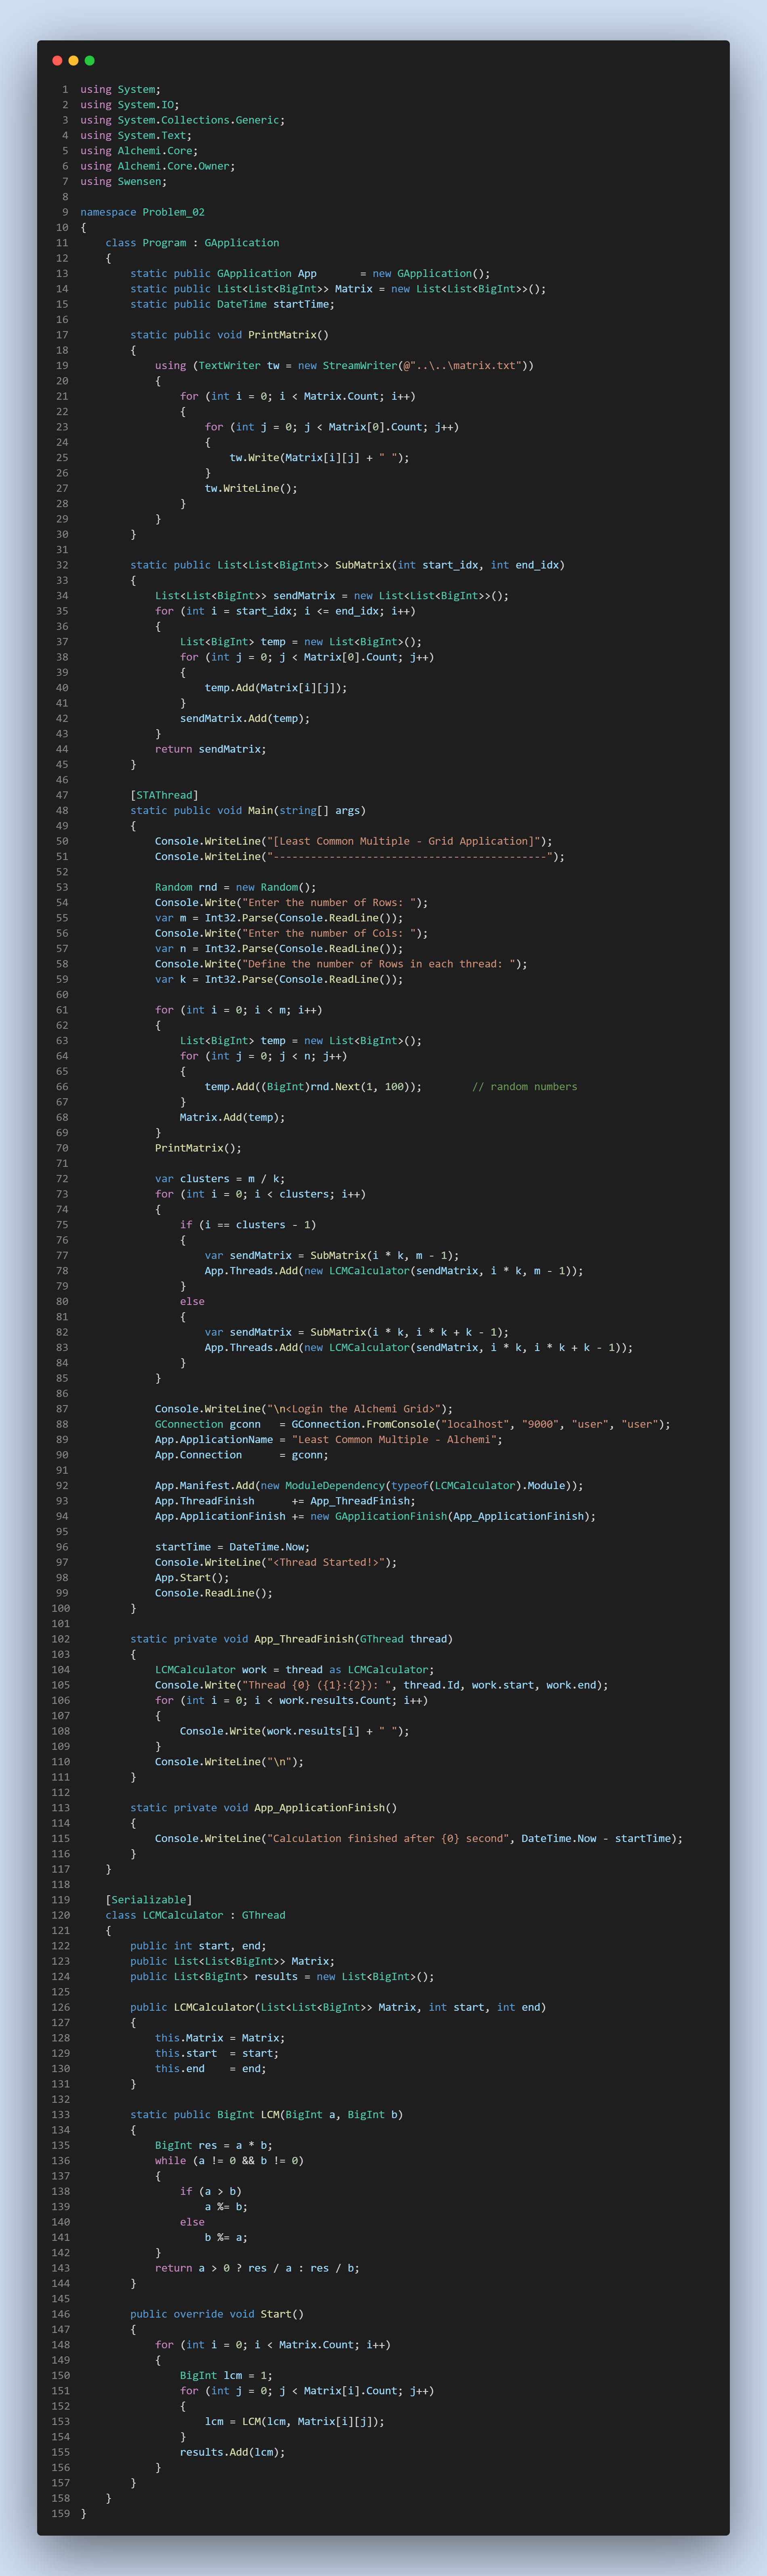
\includegraphics[trim=0in 28.2in 0in 21.25in, clip, scale=.23]{./Figures/Problem_02/Problem_02}
\clearpage
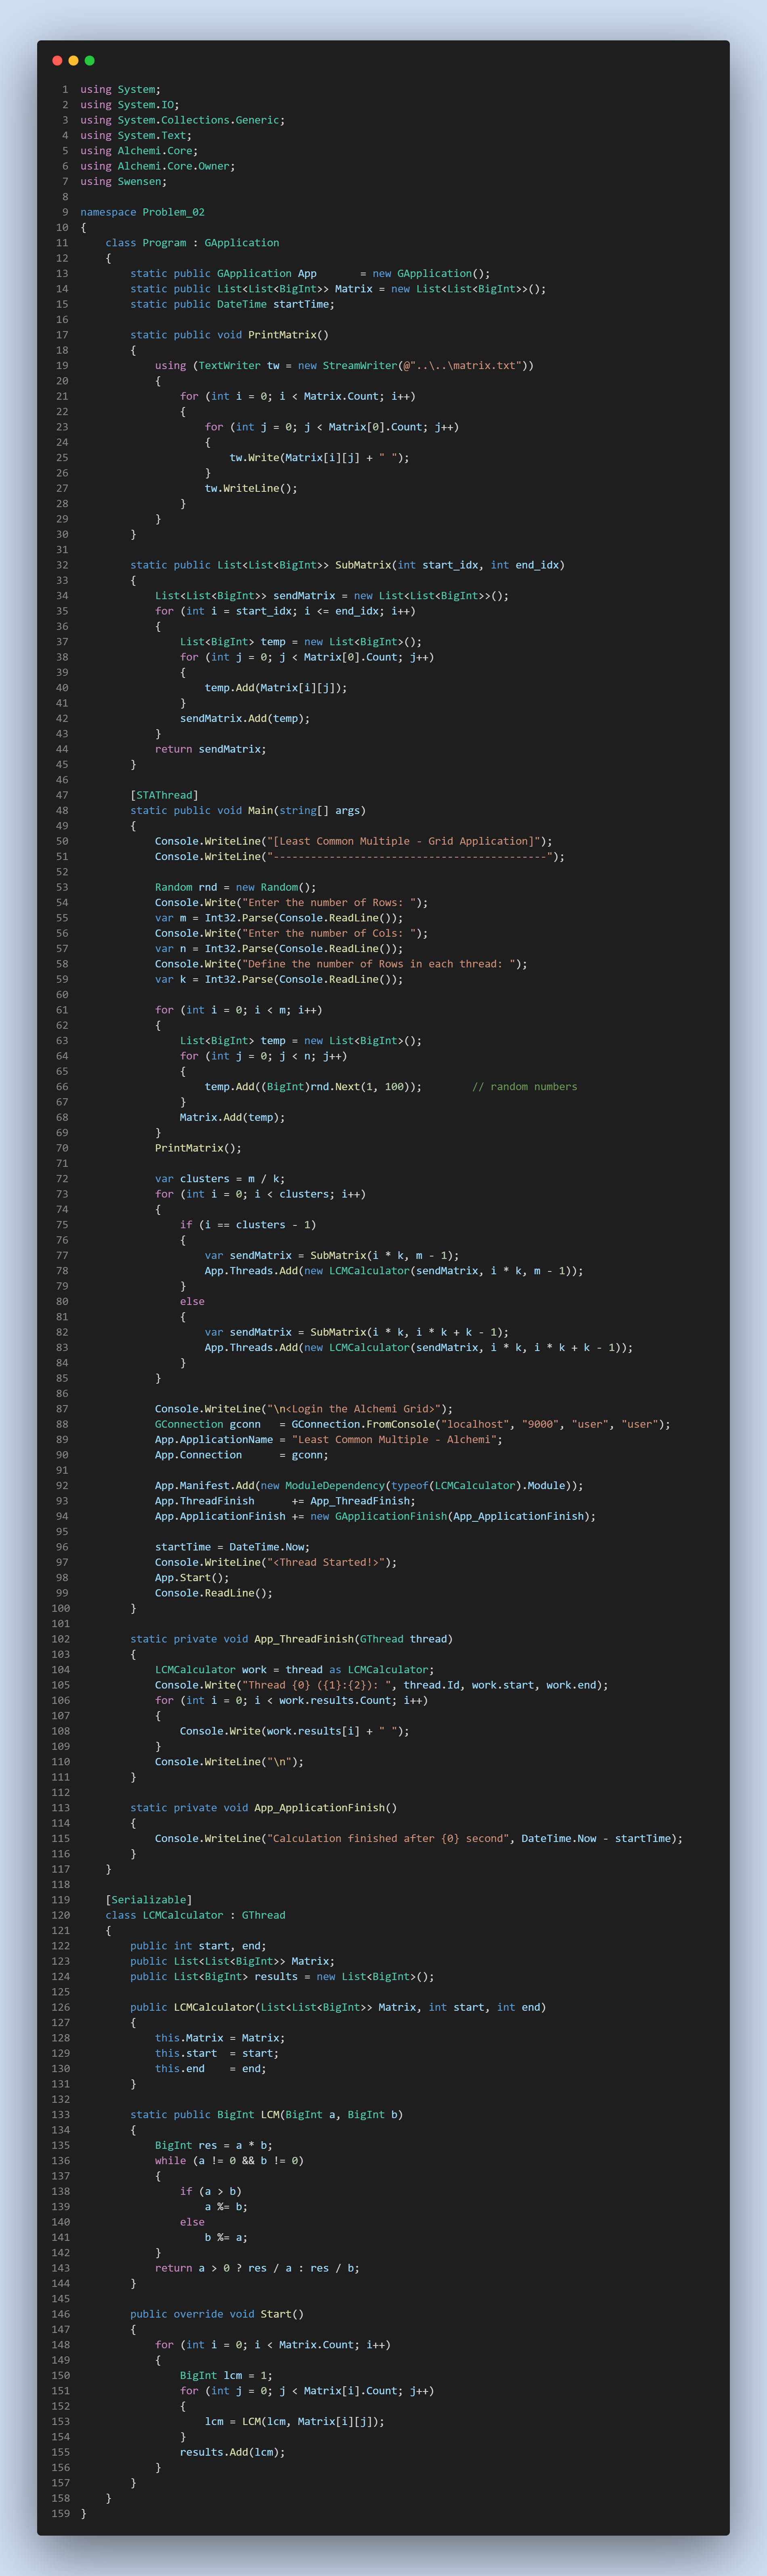
\includegraphics[trim=0in 0in 0in 60.3in, clip, scale=.23]{./Figures/Problem_02/Problem_02}
\clearpage
\end{center}

\section{Kết quả tính toán}
\begin{center}
    \begin{figure}[htp]
    \begin{center}
     	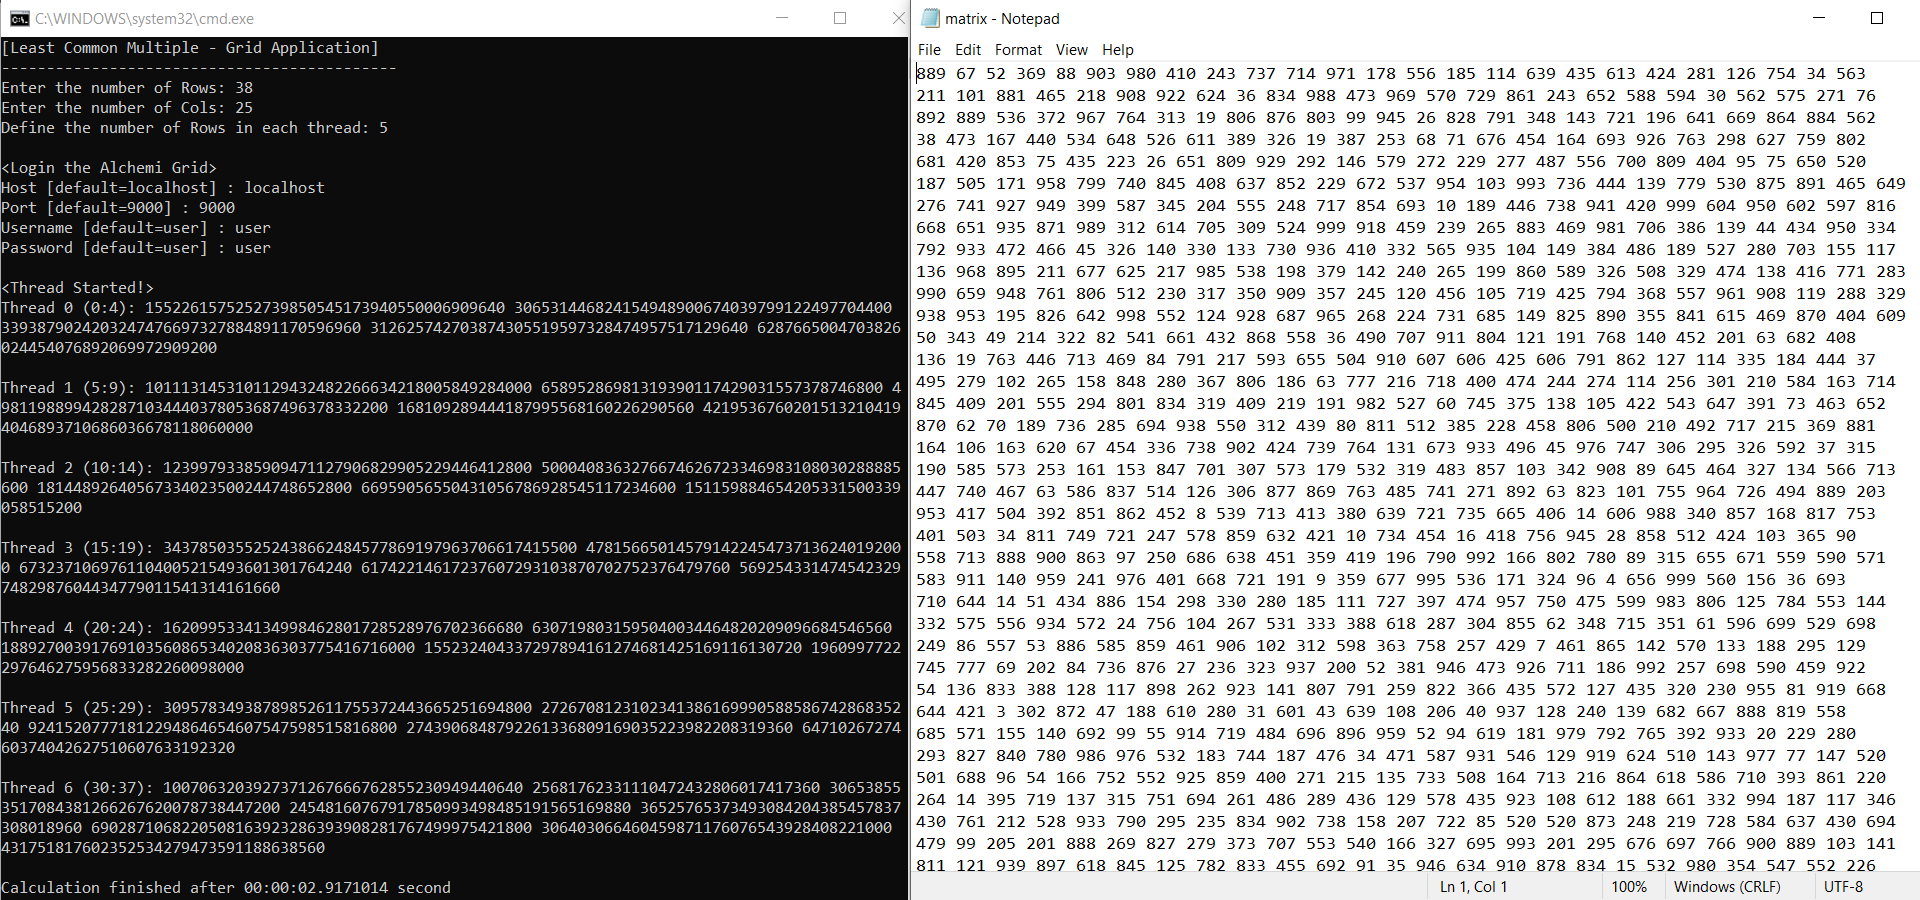
\includegraphics[trim=0in 0in 0in 0in, clip, scale=.38]{./Figures/Problem_02/Res_Problem_02}
     	\caption{Thử nghiệm với ma trận nhỏ}
    \end{center}
    \end{figure}
\end{center}

\begin{figure}[htp]
\centering
\begin{subfigure}{.5\textwidth}
  \centering
  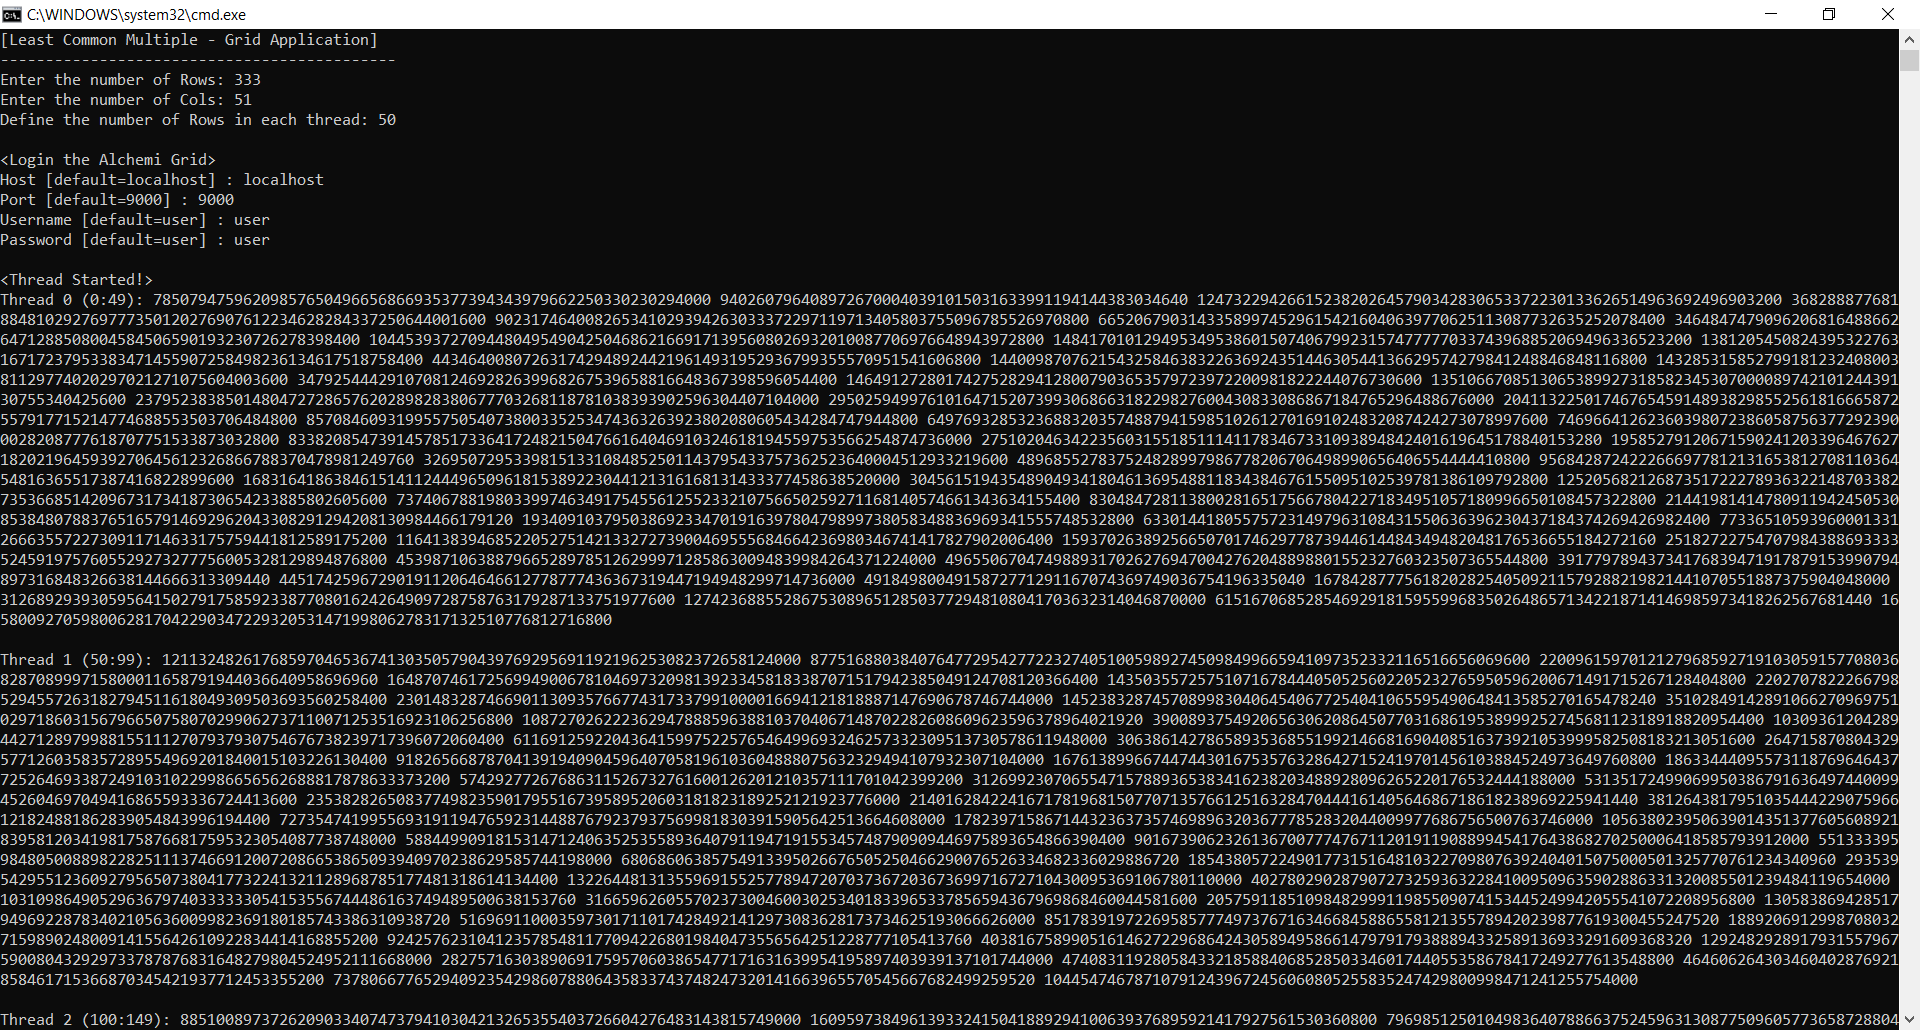
\includegraphics[width=\linewidth]{./Figures/Problem_02/Result_01}
  \label{fig:sub1}
\end{subfigure}%
\begin{subfigure}{.5\textwidth}
  \centering
  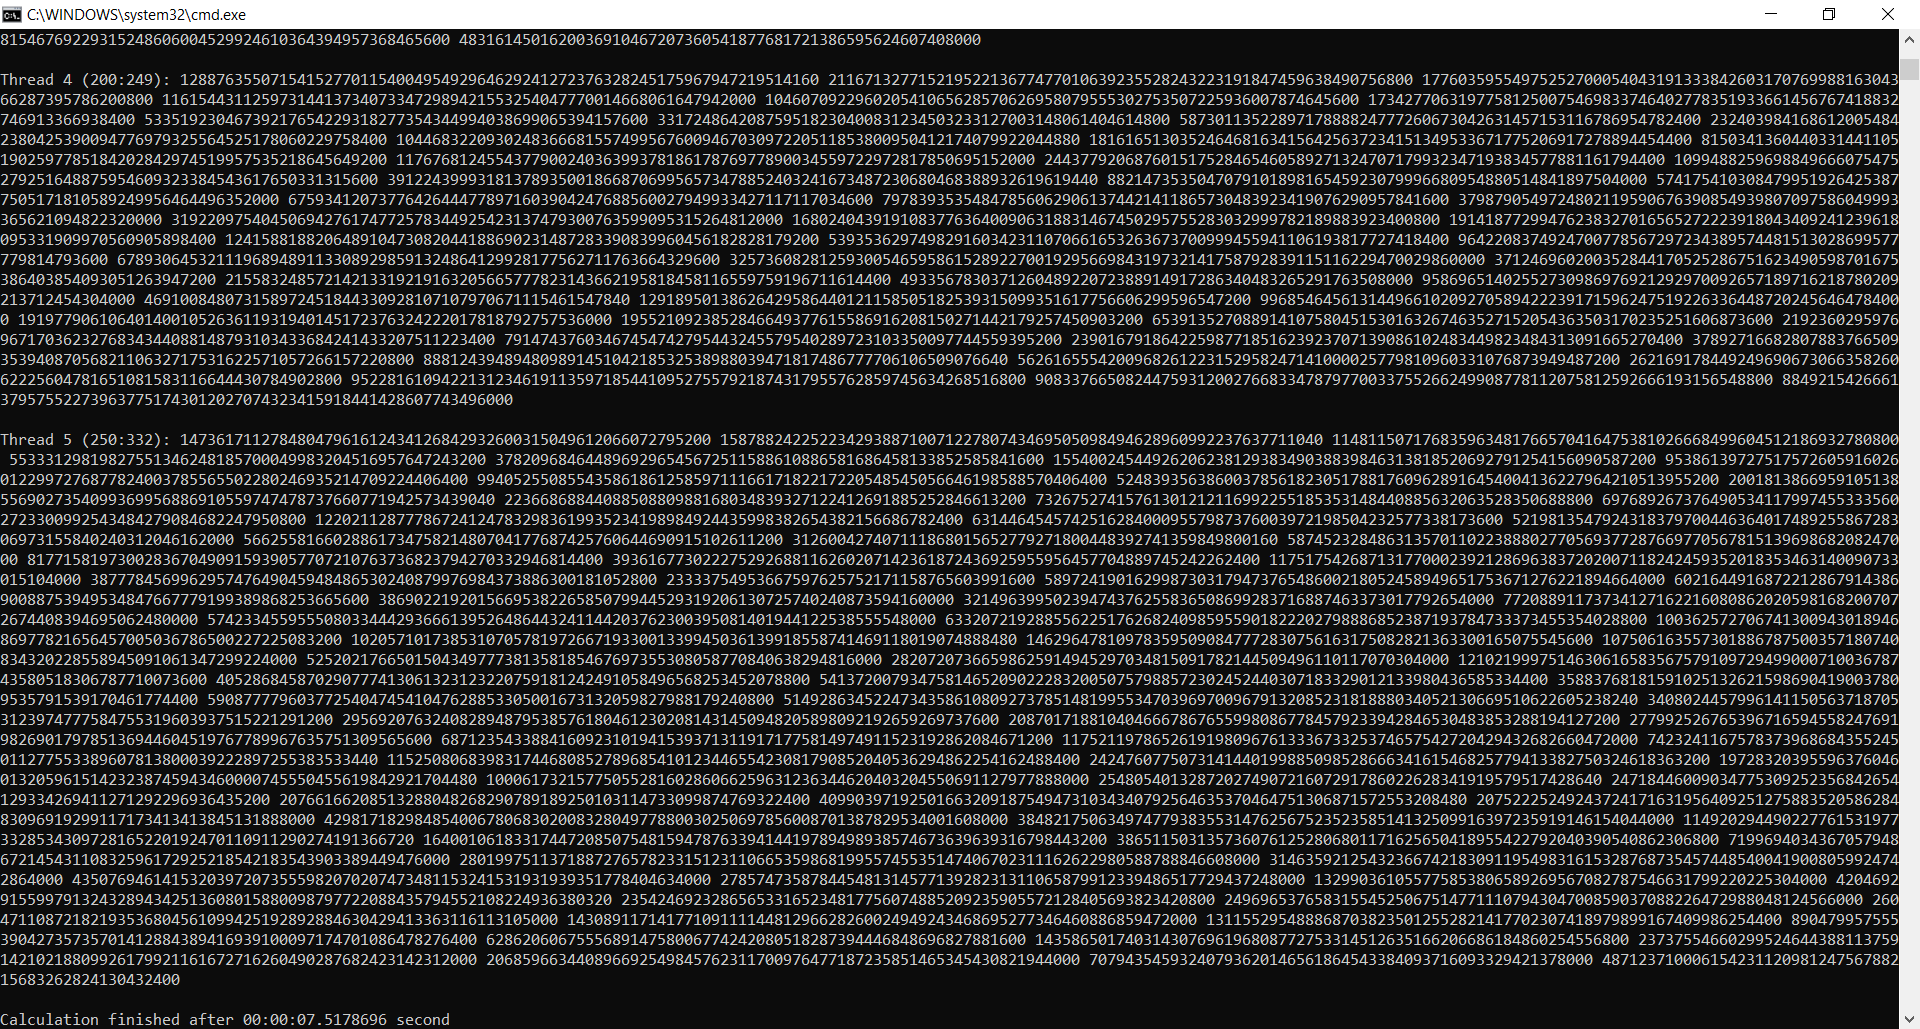
\includegraphics[width=\linewidth]{./Figures/Problem_02/Result_02}
  \label{fig:sub2}
\end{subfigure}
\caption{Thử nghiệm với ma trận lớn}
\label{fig:test}
\end{figure}

\clearpage
\section{Giao diện Alchemi}
\begin{center}
    \begin{figure}[htp]
    \begin{center}
     	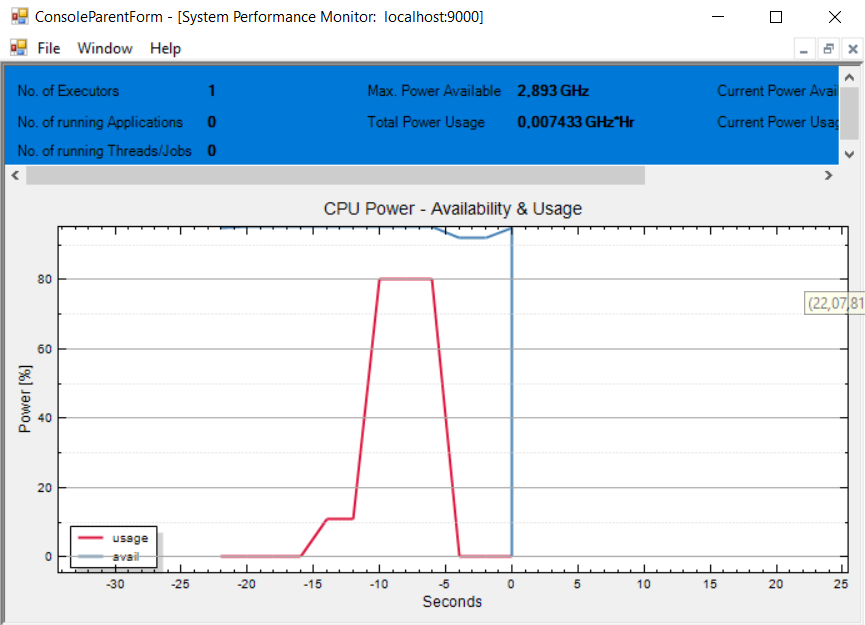
\includegraphics[scale=.56]{./Figures/Problem_02/Graph}
     	\caption{Đồ thị đánh giá hiệu năng}
  
     	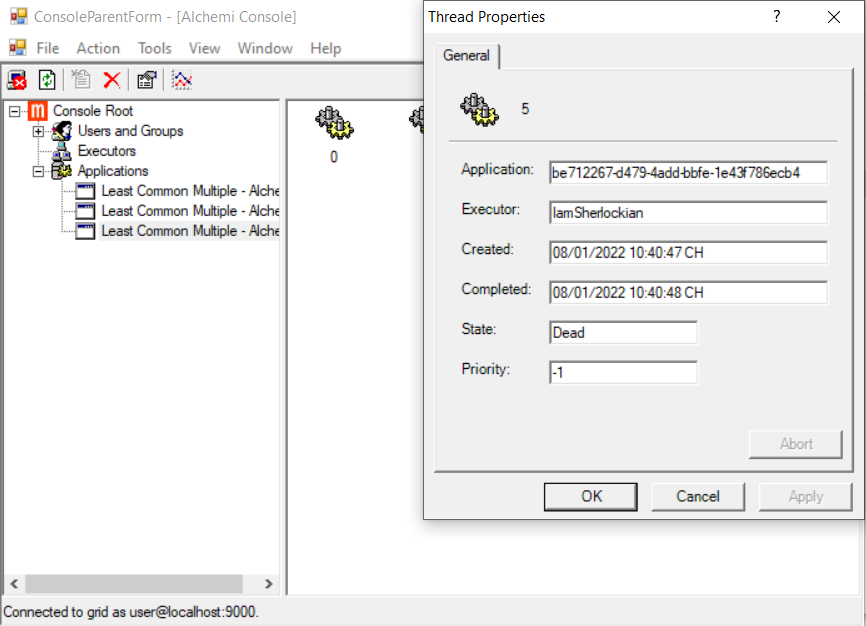
\includegraphics[scale=.56]{./Figures/Problem_02/Manage}
    	\caption{Giao diện quản lý luồng trong Alchemi Grid}
    \end{center}
    \end{figure}
\end{center}

\chapter{Số Fibonacci}

\begin{tcolorbox}[title=Đề bài, colback=red!5!white, colframe=red!70!black]
Liệt kê dãy Fibonacci đến số n cho trước (n - nhập từ bàn phím).
\end{tcolorbox}

\begin{center}
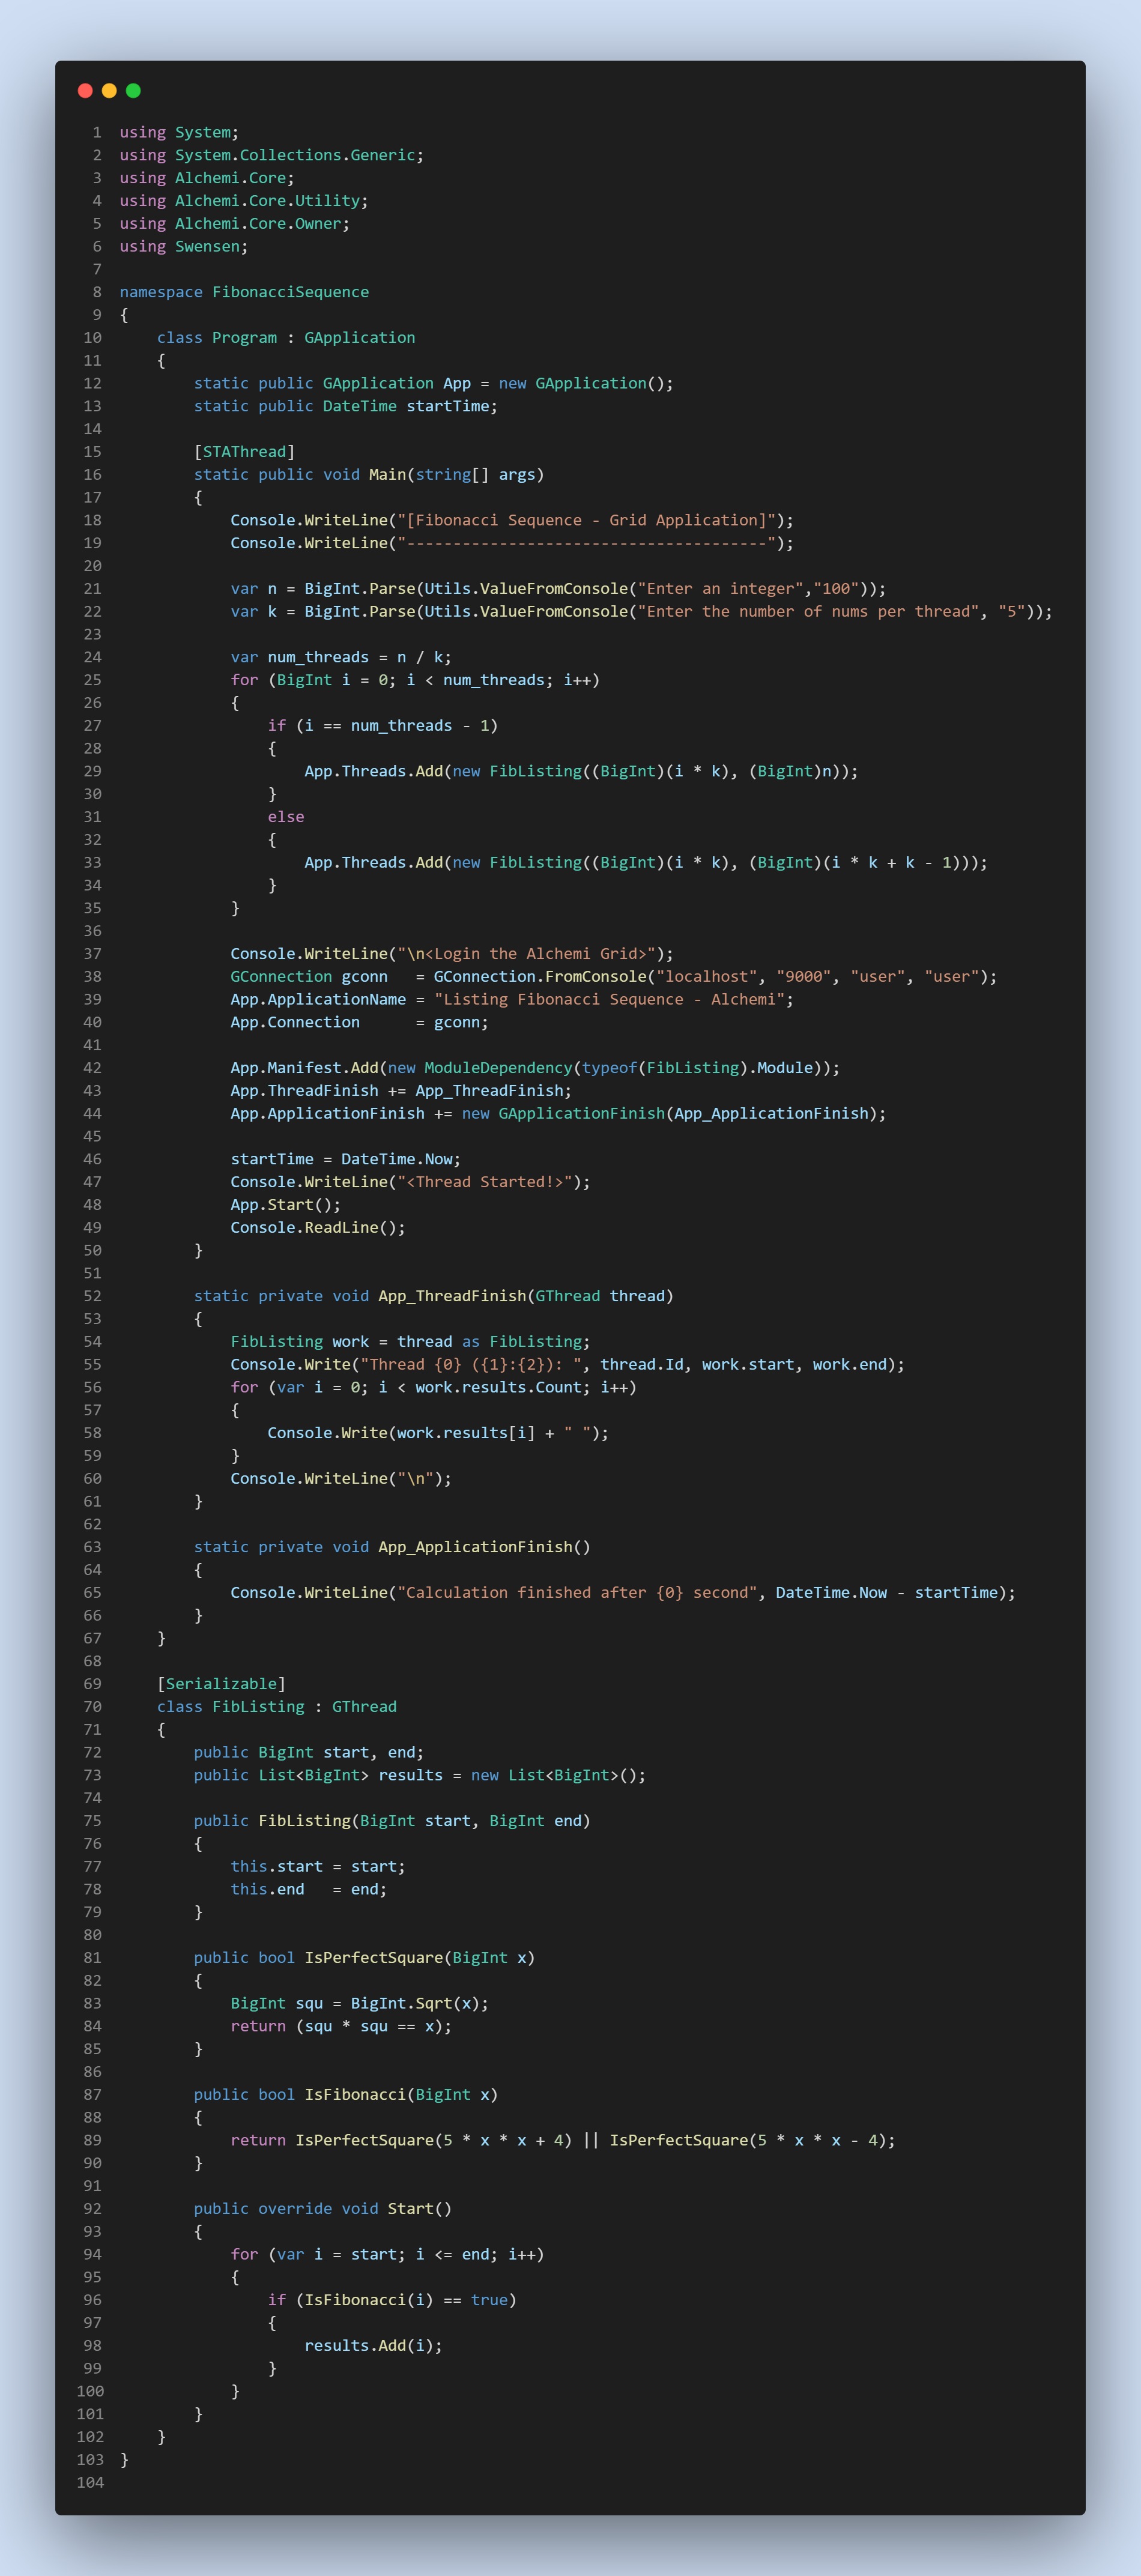
\includegraphics[trim=0in 35.1in 0in 0in, clip, scale=.23]{./Figures/FibonacciSequence/FibonacciSequence}
\clearpage
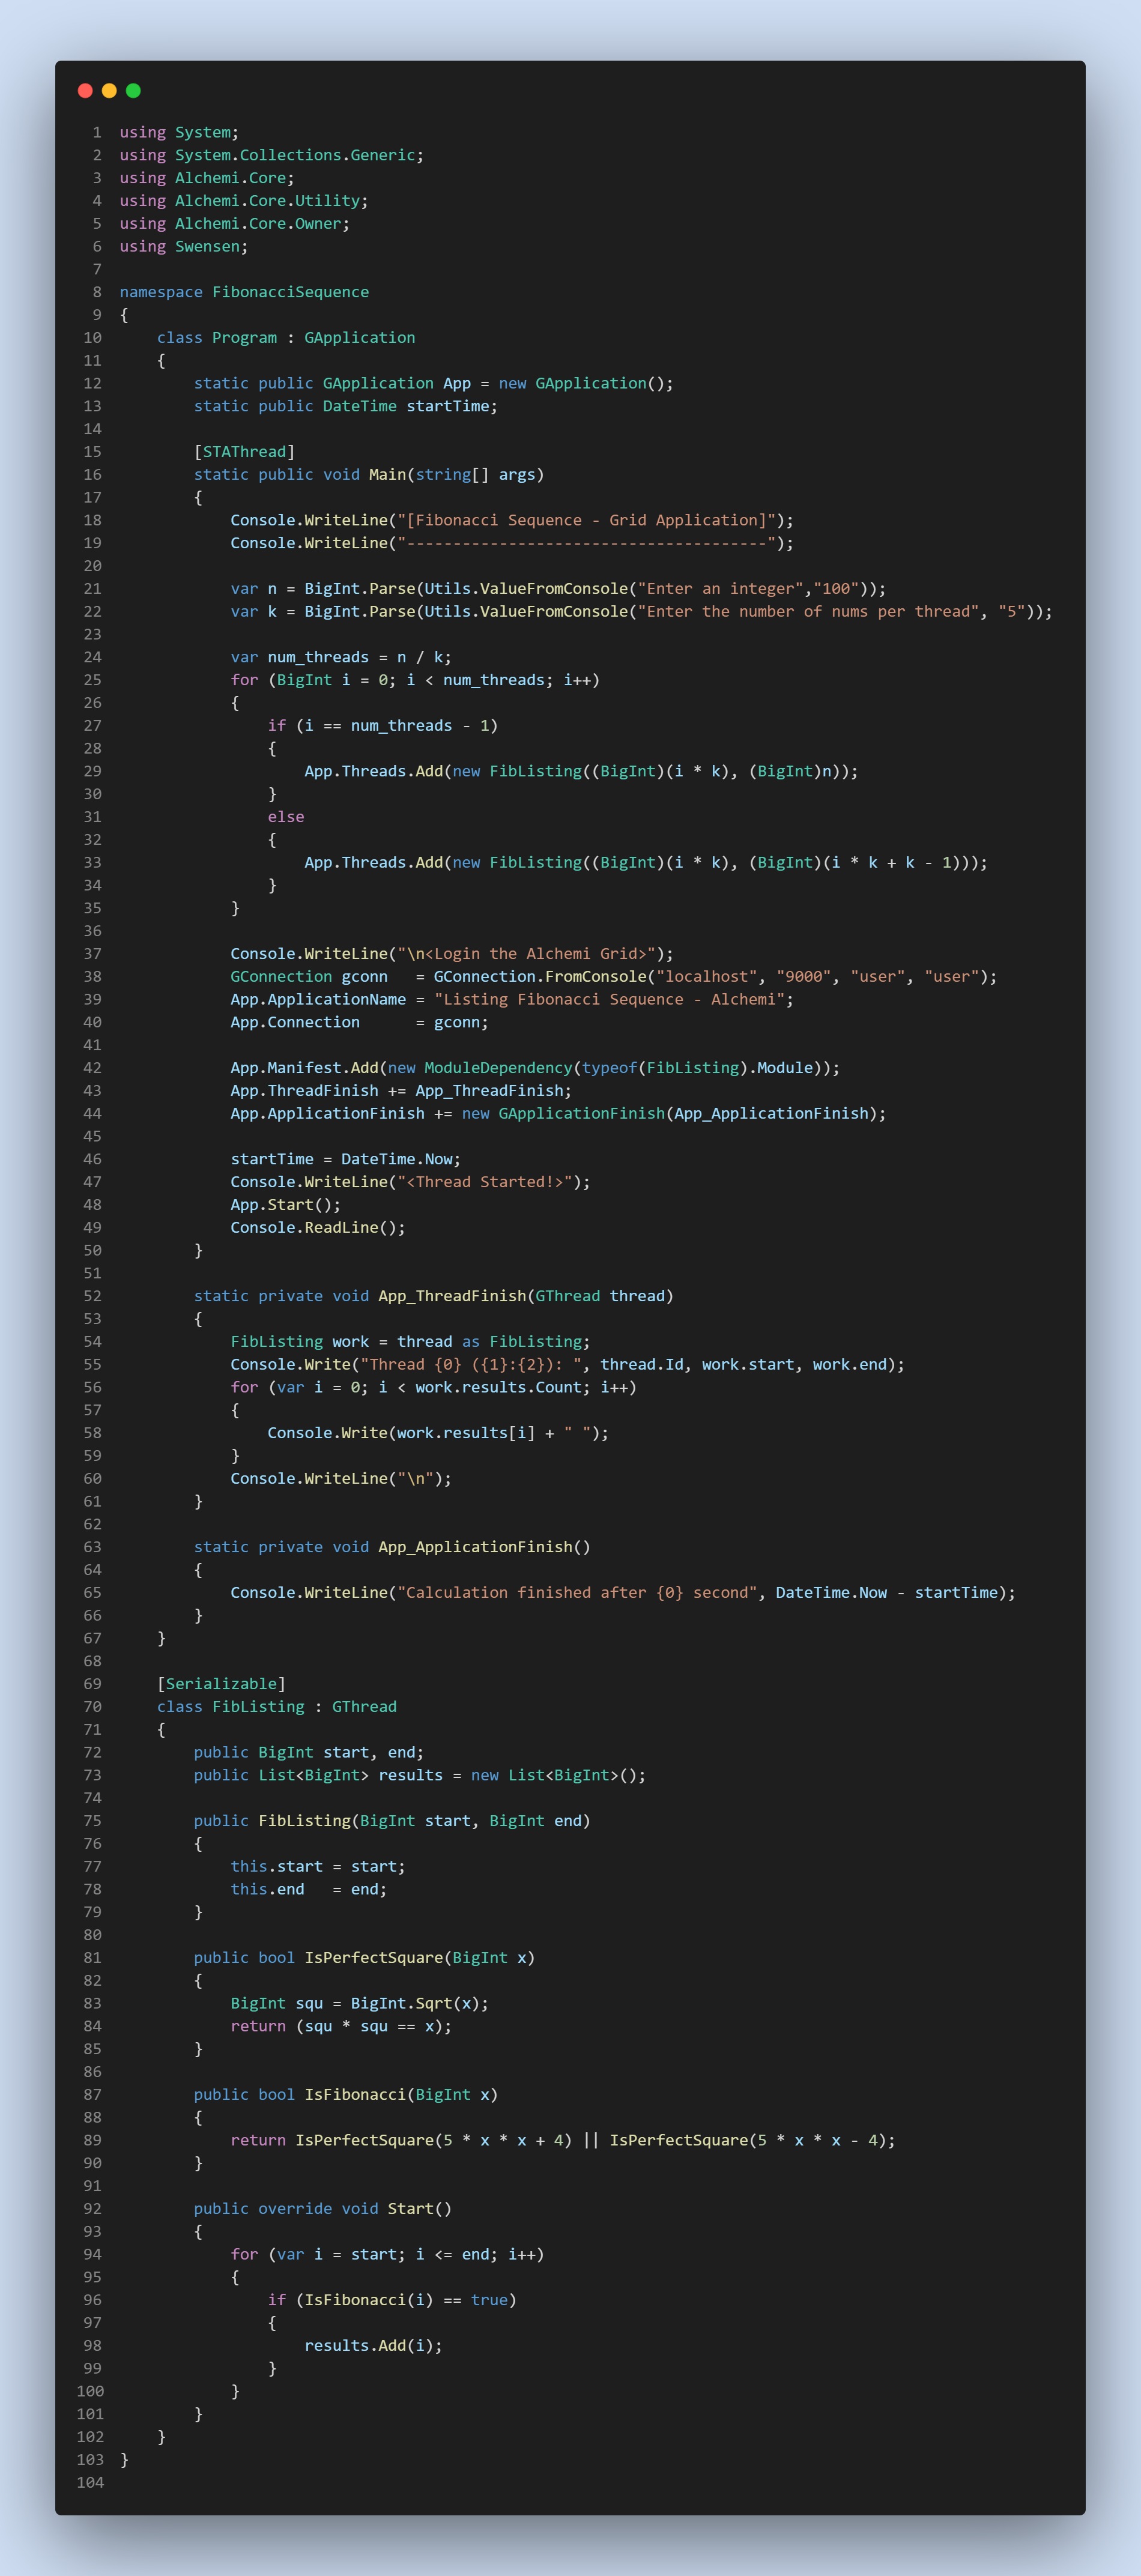
\includegraphics[trim=0in 0in 0in 24.3in, clip, scale=.23]{./Figures/FibonacciSequence/FibonacciSequence}
\clearpage
\end{center}

\section{Kết quả tính toán}
\begin{center}
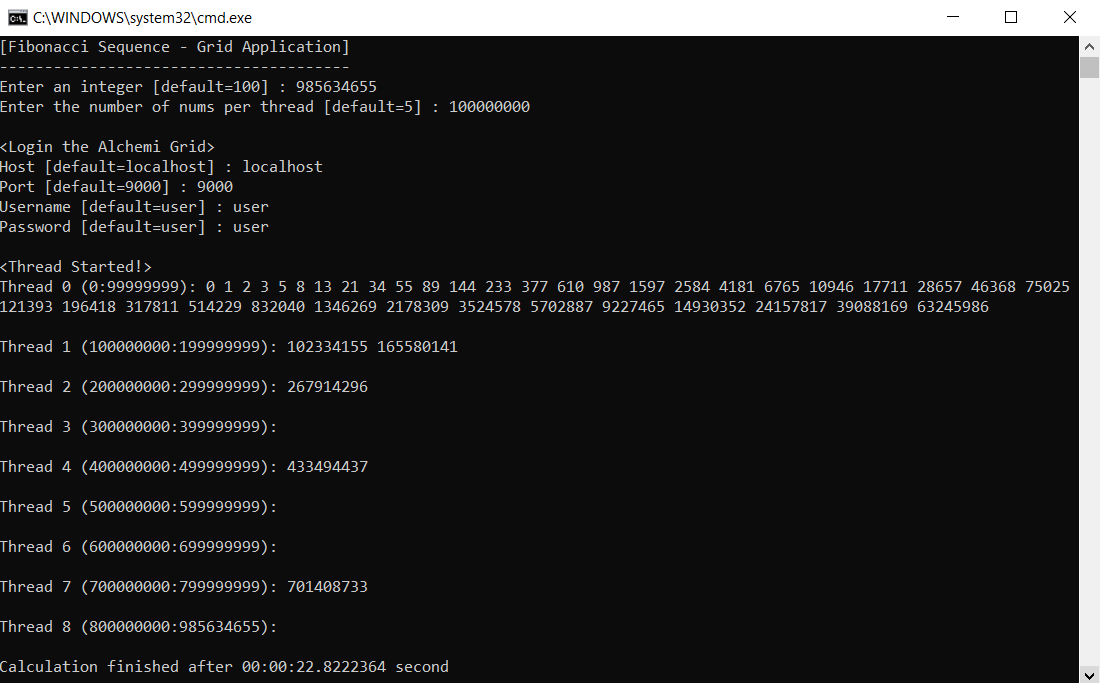
\includegraphics[scale=.6]{./Figures/FibonacciSequence/Res_FibonacciSequence}
\clearpage
\end{center}

\clearpage
\section{Giao diện Alchemi}
\begin{center}
    \begin{figure}[htp]
    \begin{center}
     	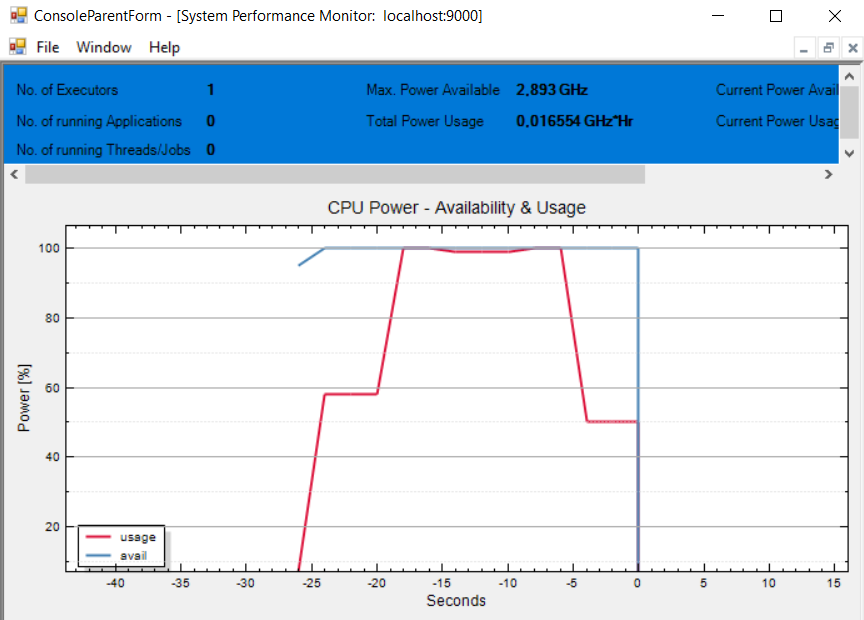
\includegraphics[scale=.6]{./Figures/FibonacciSequence/Graph}
     	\caption{Đồ thị đánh giá hiệu năng}
  
     	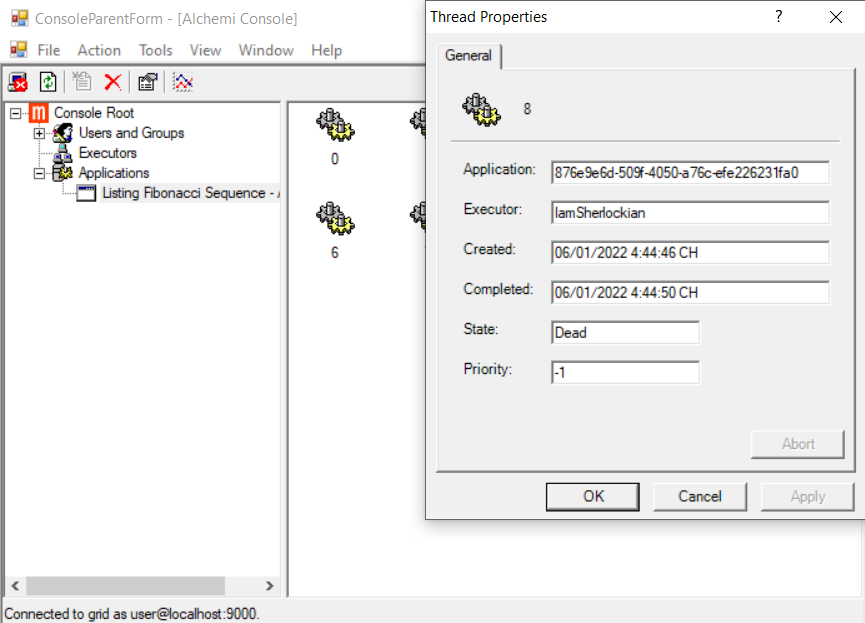
\includegraphics[scale=.6]{./Figures/FibonacciSequence/Manage}
    	\caption{Giao diện quản lý luồng trong Alchemi Grid}
    \end{center}
    \end{figure}
\end{center}


\chapter*{Kết luận}                         % Chương 3
\addcontentsline{toc}{chapter}{{\bf  Kết luận}\rm}
Với sự hướng dẫn tận tình của thầy Đoàn Duy Trung, em đã hoàn thành bài báo cáo này với hi vọng bản thân sẽ được tiếp cận tới một trong những kỹ thuật quan trọng nhất trong lĩnh vực toán-tin, công nghệ thông tin, tối ưu, ... Và giúp rèn luyện tư duy song song hóa, không chỉ có thể đưa ra lời giải cho một bài toán mà còn có thể phân tích, chia thành nhiều bài toán nhỏ để giải quyết đồng thời.

Do thời gian có hạn và khả năng còn hạn chế, bài báo cáo có thể không được hoàn chỉnh và sai sót là không tránh khỏi. Rất mong thầy và các bạn đọc bài báo cáo này có thể đóng góp ý kiến. Em xin cảm ơn!


\begin{thebibliography}{99}               % Tài liệu tham khảo   
\addcontentsline{toc}{chapter}{{\bf  Tài liệu tham khảo}\rm} 
\bibitem{pp} Slide lập trình Alchemi của thầy Đoàn Duy trung.
\bibitem{Web} https://sourceforge.net/projects/alchemi/
\bibitem{Web} https://arxiv.org/ftp/cs/papers/0402/0402017.pdf
\bibitem{Web} https://www.codeproject.com/Articles/36323/BigInt
% Chú thích: mỗi tài liệu là một bibitem.

\end{thebibliography}


\end{document}

%Một số chú ý:
%-Sau phần \end{document} thì văn bản không còn hiển thị.
%-Các siêu liên kết (tên PT, định lí... được tham chiếu) thường có ô vuông đỏ bao quanh. Các bạn yên tâm, khi in ra sẽ ko xuất hiện cái ô vuông đó!